%%%%%%%%%%%%%%%%%%%%%%%%%%%%%%%%%%%%%%%%%%%%%%%%%%%%%%%%%%%%%%%%%%%%%%
%
% Template per Elaborato di Laurea
% DISI - Dipartimento di Ingegneria e Scienza dell’Informazione
%
% update 2015-09-10
%
% Per la generazione corretta del 
% pdflatex nome_file.tex
% bibtex nome_file.aux
% pdflatex nome_file.tex
% pdflatex nome_file.tex
%
%%%%%%%%%%%%%%%%%%%%%%%%%%%%%%%%%%%%%%%%%%%%%%%%%%%%%%%%%%%%%%%%%%%%%%

% formato FRONTE RETRO
\documentclass[epsfig,a4paper,12pt,titlepage,twoside,openany]{book}
\usepackage{epsfig}
\usepackage{plain}
\usepackage{setspace}
\usepackage[paperheight=29.7cm,paperwidth=21cm,outer=1.5cm,inner=2.5cm,top=2cm,bottom=2cm]{geometry} % per definizione layout
\usepackage{titlesec} % per formato custom dei titoli dei capitoli

% Packeage added by me:
\usepackage{hyperref}	%the reference are links and not only numbers
%\usepackage[hidelinks]{hyperref} %usethis option to remove coloured rectangles around the reference (useful for print the PDF)
%NB: first we need to include hyperref and only after cleverref
\usepackage{cleveref}	%allow the use of \Cref to refer to elements

%useful for side by side images display
\usepackage{graphicx}
\usepackage{caption}
\usepackage{subcaption}

\usepackage[shortlabels]{enumitem} %enumerate with letters

%new commands
\newcommand{\bb}[0]{bounding box}

%%%%%%%%%%%%%%%%%%%%%%%%%%%%%%%%%%%%%%%%%%%%%%%%%%%%%%%%%%%%%%%%%%%%%%
% supporto lettere accentate
% 
% NB: non so perchè ma anche essendo su windows il pacchetto per windows non funziona, bisogna utilizzare quello di linux per non avere errori...
%\usepackage[latin1]{inputenc} % per Windows; 
\usepackage[utf8x]{inputenc} % per Linux (richiede il pacchetto unicode);
%\usepackage[applemac]{inputenc} % per Mac.

\singlespacing

%\usepackage[italian]{babel}

\begin{document}

  % nessuna numerazione
  \pagenumbering{gobble} 
  \pagestyle{plain}

\thispagestyle{empty}

\begin{center}
  \begin{figure}[h!]
    \centerline{
\psfig{file=logo_unitn.pdf,width=0.6\textwidth}}
  \end{figure}

  \vspace{0.5 cm} 

  \LARGE{Dipartimento di Ingegneria e Scienza dell’Informazione\\}

  \vspace{1.5 cm} 
  \Large{Corso di Laurea Magistrale in\\}
  \huge{\textbf{Computer Science and Technologies}}

  \vspace{2 cm} 
  \Large\textsc{Elaborato finale\\} 
  \vspace{0.7 cm} 
  \Huge
  	Integration of multiple deep learning algorithms\\
  	for real-time single person long-term tracking \\
  	over complex scenarios\\
  %\Large{\it{Sottotitolo (titolo definitivo???)}}


  \vspace{2 cm} 
  \begin{tabular*}{\textwidth}{ c @{\extracolsep{\fill}} c }
  \Large{Relatore} & \Large{Laureando}\\
  \Large{Luigi Palopoli}& \Large{\textbf{Stefano Leonardi}}\\
  \\
  \Large{Supervisore} & \Large{Supervisore}\\
  \Large{Stefano Divan}& \Large{Fabiano Zenatti}\\
  \end{tabular*}


  \vspace{1.5 cm} 

  \Large{Anno accademico 2019/2020}
  
\end{center}



  \clearpage
 
%%%%%%%%%%%%%%%%%%%%%%%%%%%%%%%%%%%%%%%%%%%%%%%%%%%%%%%%%%%%%%%%%%%%%%
%%%%%%%%%%%%%%%%%%%%%%%%%%%%%%%%%%%%%%%%%%%%%%%%%%%%%%%%%%%%%%%%%%%%%%
%% Nota
%%%%%%%%%%%%%%%%%%%%%%%%%%%%%%%%%%%%%%%%%%%%%%%%%%%%%%%%%%%%%%%%%%%%%%
%% Sezione Ringraziamenti opzionale
%%%%%%%%%%%%%%%%%%%%%%%%%%%%%%%%%%%%%%%%%%%%%%%%%%%%%%%%%%%%%%%%%%%%%%
%%%%%%%%%%%%%%%%%%%%%%%%%%%%%%%%%%%%%%%%%%%%%%%%%%%%%%%%%%%%%%%%%%%%%%
  \thispagestyle{empty}

\begin{center}
  {\bf \Huge Ringraziamenti (Acknowledgements)}
\end{center}
\vspace{2.5cm}
\emph{Mentre scrivo queste parole giungendo infine alla laurea, mi rendo conto di quanto sia stato lungo questo percorso accademico iniziato cinque anni fa. Da quando ho cominciato innumerevoli sono le persone che m'hanno supportato. C'è chi ha fatto parte solo di una parentesi della mia vita e chi fin dagli albori non è mai mancato. Ora che ho raggiunto questo grande traguardo vorrei ringraziarvi tutti.\\
Un grazie ai compagni di studi con cui ho condiviso le gioie e le fatiche nell'affrontare scogli sempre strani e complessi. Ringrazio quegli amici che, conosciuti in Finlandia, forse non leggeranno mai queste parole, thank you. Grazie agli amici più cari con cui condivido le più stravaganti passioni che sempre e comunque riescono a farmi sorridere e star bene. Altrettanto ringrazio i parenti a cui molto sono legato.\\
\\
Per finire vorrei ringraziare chi ha direttamente contribuito a realizzare questo lavoro di tesi. Elena per la paziente e minuziosa revisione linguistica dei contenuti. Il professor Luigi Palopoli per la sua preziosa guida. Stefano e Fabiano per la semplicità con cui in ogni momento hanno saputo consigliarmi su come affrontare questo complesso progetto complicato dal periodo che noi tutti stiamo vivendo.}

  \clearpage
  %\pagestyle{plain} % nessuna intestazione e pie pagina con numero al centro

  
  % inizio numerazione pagine in numeri arabi
  \mainmatter

%%%%%%%%%%%%%%%%%%%%%%%%%%%%%%%%%%%%%%%%%%%%%%%%%%%%%%%%%%%%%%%%%%%%%%
%%%%%%%%%%%%%%%%%%%%%%%%%%%%%%%%%%%%%%%%%%%%%%%%%%%%%%%%%%%%%%%%%%%%%%
%% Nota
%%%%%%%%%%%%%%%%%%%%%%%%%%%%%%%%%%%%%%%%%%%%%%%%%%%%%%%%%%%%%%%%%%%%%%
%% Si ricorda che il numero massimo di facciate e' 30.
%% Nel conteggio delle facciate sono incluse 
%%   indice
%%   sommario
%%   capitoli
%% Dal conteggio delle facciate sono escluse
%%   frontespizio
%%   ringraziamenti
%%   allegati    
%%%%%%%%%%%%%%%%%%%%%%%%%%%%%%%%%%%%%%%%%%%%%%%%%%%%%%%%%%%%%%%%%%%%%%
%%%%%%%%%%%%%%%%%%%%%%%%%%%%%%%%%%%%%%%%%%%%%%%%%%%%%%%%%%%%%%%%%%%%%%

    % indice
    \tableofcontents
    \clearpage
    
    
          
    % gruppo per definizone di successione capitoli senza interruzione di pagina
    \begingroup
      % nessuna interruzione di pagina tra capitoli
      % ridefinizione dei comandi di clear page
      %\renewcommand{\cleardoublepage}{} %no text in this page
      %\renewcommand{\clearpage}{} %no text until next odd page
      % redefinizione del formato del titolo del capitolo
      % da formato
      %   Capitolo X
      %   Titolo capitolo
      % a formato
      %   X   Titolo capitolo
      
      \titleformat{\chapter}
        {\normalfont\Huge\bfseries}{\thechapter}{1em}{}
        
      \titlespacing*{\chapter}{0pt}{0.59in}{0.02in}
      \titlespacing*{\section}{0pt}{0.20in}{0.02in}
      \titlespacing*{\subsection}{0pt}{0.10in}{0.02in}
      
%%%%%%%%%%%%%%%%%%%%%%%%%%%%%%%%%%%%%%%%%%%%%%%%%%%%%%%%%%%%%%%%%%%%%%
%%%%%%%%%%%%%%%%%%%%%%%%%%%%%%%%%%%%%%%%%%%%%%%%%%%%%%%%%%%%%%%%%%%%%%
%% Nota
%%%%%%%%%%%%%%%%%%%%%%%%%%%%%%%%%%%%%%%%%%%%%%%%%%%%%%%%%%%%%%%%%%%%%%
%% Sommario e' un breve riassunto del lavoro svolto dove si descrive 
%% l’obiettivo, l’oggetto della tesi, le metodologie e 
%% le tecniche usate, i dati elaborati e la spiegazione delle conclusioni 
%% alle quali siete arrivati.
%% Il sommario dell’elaborato consiste al massimo di 3 pagine e deve contenere le seguenti informazioni: 
%%   contesto e motivazioni
%%   breve riassunto del problema affrontato
%%   tecniche utilizzate e/o sviluppate
%%   risultati raggiunti, sottolineando il contributo personale del laureando/a
%%%%%%%%%%%%%%%%%%%%%%%%%%%%%%%%%%%%%%%%%%%%%%%%%%%%%%%%%%%%%%%%%%%%%%
%%%%%%%%%%%%%%%%%%%%%%%%%%%%%%%%%%%%%%%%%%%%%%%%%%%%%%%%%%%%%%%%%%%%%%
      
      %%%%%%%%%%%%%%%%%%%%%%%%%%%%%%%%
      % lista dei capitoli
      %
      % \input oppure \include
      %
      %\chapter*{Simple examples about latex code}
\label{cha:samples}

\section{reference samples}
\label{sec:refSamples}

\begin{figure}[!h] %simple figure
	\centering
	%or \columnwidth
	\includegraphics[width=0.3\linewidth]{images/ex1_yolo} %.jpg is useless
	\captionsetup{margin=0.5cm}	%margin from captions
	\caption{Object detection applied on a sample image.}
	\label{fig:sampleYolo}
\end{figure}

\begin{table}[h]	%simple table
	\centering
	\begin{tabular}{ll|l|ll}
		\cline{1-4}
		\multicolumn{1}{|l|}{c} & i & a & \multicolumn{1}{l|}{o} &                        \\ \hline
		\multicolumn{1}{l|}{}   & c & o & \multicolumn{1}{l|}{m} & \multicolumn{1}{l|}{e} \\ \cline{2-5} 
		\multicolumn{1}{l|}{}   & v & a &                        &                        \\ \cline{2-3}
		&   & ? &                        &                        \\ \cline{3-3}
	\end{tabular}
	\caption{Example table.}
	\label{tab:sampleTable}
\end{table}

Try to cite different elements\footnote{Not only reference but also footnote ;)}:
\begin{itemize}		%bullet point
	\item images show at: \Cref{fig:peoplePair}\\
		  more complex images can be found at: \href{https://tex.stackexchange.com/questions/37581/latex-figures-side-by-side}{side by side images}
	\item look at \Cref{tab:sampleTable}\\
	it can be generatedonline at this \href{https://www.tablesgenerator.com/}{online editor}.
	\item the sample chapter can be found at: \Cref{cha:samples}
	\item precisely at \Cref{sec:refSamples}
	\item yolov3 \cite{yoloV3}
\end{itemize}

\begin{tcolorbox}	%text area
	\begin{center}
		Nice text area :D
	\end{center}
\end{tcolorbox}

\begin{figure}		%an image with sub-images
	\centering
	\begin{minipage}{.49\textwidth}
		\centering
		\includegraphics[width=1\linewidth]{images/ex1_yolo}
		\captionof{figure}[shortcut for list of figure]{Description 1.}
		\label{fig:qqq}
	\end{minipage}
	\begin{minipage}{.49\textwidth}
		\centering
		\includegraphics[width=1\linewidth]{images/ex1_yolo}
		\captionsetup{margin=0.5cm}
		\captionof{figure}{Description 2}
		\label{fig:bbb}
	\end{minipage}
\end{figure}

\begin{figure}		%two separate images side by side
	\centering
	\begin{minipage}{.49\textwidth}
		\centering
		\includegraphics[width=1\linewidth]{images/ex1_yolo}
		\captionof{figure}{image description 1}
	\end{minipage}
	\begin{minipage}{.49\textwidth}
		\centering
		\includegraphics[width=1\linewidth]{images/ex1_yolo}
		\captionof{figure}{image description 2}
	\end{minipage}
\end{figure}
      %%%%%%%%%%%%%%%%%%%%%%%%%%%%%%%%%%%%%%%%%%%%%%%%%%%%%%%%%%%%%%%%%%%%%%
%%%%%%%%%%%%%%%%%%%%%%%%%%%%%%%%%%%%%%%%%%%%%%%%%%%%%%%%%%%%%%%%%%%%%%
%% Nota
%%%%%%%%%%%%%%%%%%%%%%%%%%%%%%%%%%%%%%%%%%%%%%%%%%%%%%%%%%%%%%%%%%%%%%
%% Sommario e' un breve riassunto del lavoro svolto dove si descrive l’obiettivo, l’oggetto della tesi, le metodologie e le tecniche usate, i dati elaborati e la spiegazione delle conclusioni alle quali siete arrivati.
%% Il sommario dell’elaborato consiste al massimo di 3 pagine e deve contenere le seguenti informazioni: 
%%   contesto e motivazioni
%%   breve riassunto del problema affrontato
%%   tecniche utilizzate e/o sviluppate
%%   risultati raggiunti, sottolineando il contributo personale del laureando/a
%%%%%%%%%%%%%%%%%%%%%%%%%%%%%%%%%%%%%%%%%%%%%%%%%%%%%%%%%%%%%%%%%%%%%%
%%%%%%%%%%%%%%%%%%%%%%%%%%%%%%%%%%%%%%%%%%%%%%%%%%%%%%%%%%%%%%%%%%%%%%
\chapter{Sommario}\label{cha:summary}
Sommario è un breve riassunto del lavoro svolto dove si descrive l'obiettivo, l'oggetto della tesi, le metodologie e le tecniche usate, i dati elaborati e la spiegazione delle conclusioni alle quali siete arrivati.  

Il sommario dell’elaborato consiste al massimo di 3 pagine e deve contenere le seguenti informazioni:
\begin{itemize}
  \item contesto e motivazioni 
  \item breve riassunto del problema affrontato
  \item tecniche utilizzate e/o sviluppate
  \item risultati raggiunti, sottolineando il contributo personale del laureando/a
\end{itemize}




		\clearpage
      \chapter{Introduction} \label{cha:introduction}
This chapter offers an overview of the project on which the thesis is based. The goal is to explain in detail how the practical problem has been approached in order to analyze the physical constraints, ideate a software method able to solve them, and how these ideas were then implemented into a working algorithm. 


\section{Physical context}
The physical component in this project is a robot. Its definition can vary a lot basing on the context in which it is used. For this project, a robot can be described as a vehicle able to move in the space. A \textbf{LIDAR (Laser Imaging Detection And Ranging)} sensor is mounted. Which allows to drive in the space avoiding physical obstacles during the movement. In addition, it is installed a computational device connected to a webcam that can record streams of images representing the space in front of the robot itself.\\
The video camera becomes the eye of the robot itself, and the captured video stream is used as the input of the algorithm working on the computational device. This computer can be composed of a \textbf{CPU (Central Processing Unit)} or more likely it is built with a \textbf{GPU (Graphics Processing Unit)} that can speed up parallelized computation, applied on the \textbf{DNNs (Deep Neural Networks)} used as the core of the algorithm. The software does not assume one component over the other, the only variation is in the performances: a GPU computation speed can be much higher than a CPU.\\
Instead, the output of the algorithm is a position composed of X and Y pixel coordinates calculated on a single frame captured from the webcam. This location can be then elaborated and, with the use of LIDAR sensor, the robot can estimate which is the 3D position of the element tracked from the software.\\
Finally, it moves to reach that position, in order to follow the tracked subject not only into the virtual space but also into the real environment.


\section{The Problem}
The thesis project is based on an internship with Dolomiti Robotics\cite{dolomitiRobotics}, a company working on self-driving robots.\\
These vehicles are designed to work in an industrial environment. This scenario is populated not only by robots but also people, making the driving task even more complex to achieve.

\subsection{Robot only environment}
A completely automated environment, where humans cannot access looks to be a similar context. Instead, it is completely different because each vehicle has is its own logic that can be designed to fit the requirements of all the other robots working in that area.\\
The typical solutions to drive a vehicle in this scenario are two:
\begin{itemize}
	\item Based on a centralized decision unit that moves all the robots simultaneously around. This unit is responsible for avoiding collisions by knowing the exact position of each single moving robot.
	\item Based on fixed rules of movement that each robot has to follow. The rules do not allow collision and the automated vehicles respect them.
\end{itemize}
Both these methods work because an automated vehicle uses a deterministic decision process and does not take arbitrary choices.

\subsection{Environment shared between robots and humans}
Instead, in a shared environment, there are a lot of elements that are not controlled by a deterministic rule. The changes in the scenario are random and prediction cannot be done. There are both fixed object that may have changed position due to external interaction, and also human that walk around with no defined rules.\\
In this scenario, it is fundamental to choose an input method that can measure the area around, in order to create an autonomous moving vehicle. Therefore LIDAR has been chosen. LIDAR is a technology that measures distances around the robot in a horizontal plane. The effect is that the robot knows in each direction which is the distance from the surrounding objects. This key idea has been used from Dolomiti Robotics, to design a software able to drive robots around avoiding collision with fixed obstacles or people walking.\\
While a robot moves around, it can construct a map of the fixed objects in the environment, measured with LIDAR. Instead, the moving objects, such as other robots or people, that are recognised as not fixed elements are not stored in the map as obstacles. This reconstruction allows the vehicle to move autonomously from one position to another knowing exactly which path to follow to reach the destination.

\subsection{Purpose of the internship}
The shared environment does not offer any real human-robot exchange. The two parts only share the same spaces. The purpose of this thesis project is to create a physical interaction between the two.\\
The goal is to create a new functionality \textit{"that allows a robot to follow a person into the real environment"}. How it works:
\begin{itemize}
	\item Track/follow is the interaction of a robot and a single person (called from now on \textbf{Leader}).
	\item The Leader starts the \textit{"follow"} functionality standing in front of the webcam of the robot.
	\item The robot has few seconds to recognise the person inside the camera \textbf{FOV (Field Of View)} as the Leader.
	\item Then the Leader can freely move around in the space. 
	\item In the meanwhile the algorithm is processing the webcam stream of images recognising the position of the Leader and start tracking it in the virtual space, while following it in the real one.
	\item The tracking continues for a long period, up to minutes until this functionality is stopped.
\end{itemize}

\subsection{Technical problems}\label{sec:technicalProblems}
This "follow" functionality may be easily solved under certain conditions. However, solving the general scenario, it is a much harder task.\\
Below is listed a small collection of the principal problems that make this functionality an extremely general one, therefore hard to solve.
\begin{itemize}
	\item The tracking should be done in real-time. It is impossible to follow a person if the processing speed is too slow. A high \textbf{FPS (Frames Per Second)} rate should be respected.
	\item The robot needs to physically follow the person meaning that the webcam cannot be fixed. By consequence, also the background is not fixed and the entire captured image, subject included, might be blurred.
	\item The person can move freely around walking fast, slow, or staying.
	\item The Leader is a random person, it is not known while the algorithm was designed (no parameters can be fixed in advance).
	\item While the Leader is walking around there might be also other people that interfere with the algorithm.
	\item The Leader can be hidden from the webcam due to moving or static elements placed between the Leader and the webcam itself.
	\item The Leader can exit the field of view of the webcam disappearing until the robot rotates to watch it back again.
	\item The tracking should be performed for a long period.
\end{itemize}


\section{The Solution}
The problem is complex due to its generality and the necessity to cover a lot of complementary conditions. For this reason more than one solution exists. In this thesis is presented a solution based on the combination of three methods. Each one is designed to solve sub-problem compared to this one, and none of them alone can overcome the challenge of the general task.\\

\subsection{Existing technologies}\label{sec:existingTechnologies}
The three technologies are:
\begin{itemize}
	\item \textbf{Object Detection (or Localization):} given an image the object detection task aim at processing the image and recognise which objects exist there. The detection not only need to produce a list of all the classes\footnote{There are a set of types to which each element can be associated i.e. person, dog, car, bicycle, bottle and so on.} of objects visible in the image, but also recognise in which section of the frame every single element is.\\
	The output of detection is a list of: class to which the element belongs, the probability associated and the \textbf{bounding box} defined as the smallest rectangle that contains the entire element.

	\item \textbf{Object Tracking:} in this case the input is not a single image but a video stream and an initial section\footnote{A portion of the image: a rectangle.} of it. The goal is to remember this portion of the image and recognise it in all the frames after the first one. It is important to note that the tracking procedure it is not designed to follow a person, a car or other it is designed to follow a rectangle of coloured pixels, no matter what these pixels represent.

	\item \textbf{Object Recognition:} this is a comparison between several pictures. These often represent a bounding box of the object that needs to be recognised. The procedure has a database of images each one with a specific class, and the input value is another picture, called \textbf{query}, that does not exist in the database but it represents a subject known. The goal is to extract from the database all the images that have a subject that looks similar to the one represented in the query.\\
	This application is mainly used to recognise humans, often in the video surveillance context. The database is composed of the bounding box of all the people seen, i.e. in a supermarket over the last week, and when a thief is captured and it is used as a query. So, the system should return all the images containing the thief itself.
\end{itemize}

\subsection{Limitation of known technologies}
The challenges presented previously in \Cref{sec:existingTechnologies}, can solve a small part of the general problem but each one has a technical problem~\Cref{sec:technicalProblems} that cannot be solved:
\begin{itemize}
	\item Object detection is a computationally expensive task, on a powerful GPU can run in real-time but that is not the case of the robots we are working with.\\
	In addition, the detection works frame by frame and each one is independent of the previous one. So, if a person is recognised in a frame, and in the next one, there is more than a single person the algorithm does not know the relation between all of them. Meaning that a person cannot be tracked from one frame to the next one.

	\item Object tracking, according to the name, seems the task that better match the requirement of the general problem.\\
	Despite that, the tracking does not consider that the tracked subject, the Leader, cannot be hidden from the webcam. The Leader should always be visible into the recorded video, and that is not the case. In addition, the Leader can also exit the field of view of the robot while walking around.\\
	Lastly, all the trackers are designed to follow the subject for small periods\footnote{Each tracker works on a video of few seconds.}, after a while the tracked rectangle of coloured pixel changes and the precision of the output is no more not guaranteed. This phenomenon is known as the \textbf{drift effect}, after a while the drift is so wide that the tracked cannot be trusted anymore.

	\item Object recognition due to its requirement was not designed at all to run in real-time. In fact, it is enough to run this procedure only when a query occurs, and that does not happen more than one every second.\\
	Except that, there is a more intrinsic problem with the recognition to approach the general problem. The procedure requires a query that can be the subject at the actual frame, but then it should work on a dataset composed of old frames and these are useless to solve the actual frame.\\
	In addition, this algorithm cannot be independent, because the input values are bounding boxes of people, but these regions can be computed only with an object detection algorithm. Hence this approach cannot solve the problem independently.
\end{itemize}

This explanation shows that none of the existing proposed technologies can solve the general problem in all its parts.

\subsection{Combine known methods to solve the general task}
To solve the problem and manage all the requirements it is necessary to create a combination of known methods.\\
An example of integration of methods to solve a complex task was done by Jiang et al, in their paper\cite{multi-feature-fusion-and-YOLO} that presents a fusion of \textbf{YOLO9000}\cite{yoloV2} (the second version of \textbf{YOLO}\cite{yolo}) used as object detector and \textbf{SURF}\cite{surf} used as short-term object tracker.\\
The paper illustrate an innovative approach based on two thresholds that are used to understand when the drift of the tracker is too large and it is necessary to reinitialize it. So YOLO is executed to find the tracked subject back again and after the initialization the loop can start again.\\
\\
The method presented in that paper is an integration of two class of methods. Instead in this thesis is presented an integration of three. The third method is necessary because an additional technical problem exists~(\Cref{sec:technicalProblems}). Jiang et al. work on sport video clips where athletes are always followed by the camera and never disappear out of the field of view. In addition, occlusion can exist but are very short and the tracker is often able to overcome them.\\
Instead, in our scenario we need  to manage the disappearance of the Leader behind a corner for a relatively long time. So, the object recognition method was introduced to solve this condition.\\ 
These are the main steps of the entire algorithm:
\begin{enumerate}
	\item The \underline{detection} is executed and the bounding box of the Leader is found. By assumptions, in this phase, if more than one person is simultaneously found the detections are ignored.
	\item The \underline{tracker} is initialized with the bounding box found.
	\item The tracker runs for the next F frames.
	\item A new detection is executed and D people are found.
	\item The \underline{person recognition} is used to choose if the Leader is contained in the list of people found:
	\begin{itemize}
		\item If \textbf{yes}: the procedure starts again from point 2 (tracking)
		\item If \textbf{not}: the procedure loops again from point 4 (detection again)
	\end{itemize}
\end{enumerate}

This flow shows how detection, tracking and recognition are combined together to build a complete algorithm, that can run in real-time due to the alternation of slow and fast methods and to manage all the problematic scenarios.\\
The details will follow.

\section{Structure of the thesis}
The next chapters are organized as follows. This section concludes the introduction (\Cref{cha:introduction}).\\
Then follow three chapters one for each main method: object detection in~\Cref{cha:detection}, object tracking in~\Cref{cha:tracking} and object recognition in~\Cref{cha:recognition}.\\
An overview of the entire algorithm and how it works together follow  in~\Cref{cha:solution}.\\
In the end, the conclusions are presented in~\Cref{cha:conclusions}.





\clearpage
      \chapter{Object Detection} \label{cha:detection}
This chapter explains into details what is the object detection task and the methods that can solve it efficiently. Moreover an overview of other methods is given among whose there not efficient ones and others that may seem to solve the task but do not.

\section{Task definition}
Object detection, also known as \textbf{object localization}, is an evolution of the \textbf{image classification} (\Cref{fig:imgAnalysisType}). In classification, an algorithm should produce a list of all the classes of objects inside the image. Instead, the detection not only calculates which object class exists but also how many occurrences are present for each class. Then, the complex part, and the most interesting one for this thesis application, is localizing where those elements are placed inside the image. The position is not considered as a point but as a bounding box defined as the smallest rectangle that contains the entire element. An example of object detection is shown in~\Cref{fig:sampleYolo}.
\begin{figure}[!h]
	\centering
	\includegraphics[width=0.8\linewidth]{images/detection/ex1_yolo}
	\caption{Object detection applied on a sample image.}
	\label{fig:sampleYolo}
\end{figure}

\subsection{Similar tasks}
Object detection can be additionally improved to extract even more information from an image.\\
The main evolutions, shown in~\Cref{fig:imgAnalysisType} are:
\begin{itemize}
	\item \textbf{Semantic segmentation:} takes all the bounding boxes produced by an object detector, and for each one, it calculates the pixels that belong to the object itself and the ones that do not. By doing this each class has its own colour associated. As a result, the algorithm knows for each pixel if it belongs to one label associated with the image (semantic division) or to the background (yellow in the image).
	\item \textbf{Instance segmentation:} is similar to semantic segmentation, but in this case, each instance of the object is considered as a new element. In fact, the three cubes in the figure have different colours associated to them.\\
	This task is solved by the \textbf{Mask-R-CNN algorithm} (\Cref{sec:mask-r-cnn}).
	\item \textbf{(Human) pose estimation:} is the most complex task among the five. Mainly applied to people, this challenge consists in the estimation of the 3D position of the body. The idea is to build up a skeleton of the person in the image and understand how its body limbs are positioned. This functionality is important to understand what a person is doing in the image.\\
	This task is solved by the \textbf{OpenPose estimation algorithm} (\Cref{sec:openpose}).
\end{itemize}
\begin{figure}[!h]
	\centering
	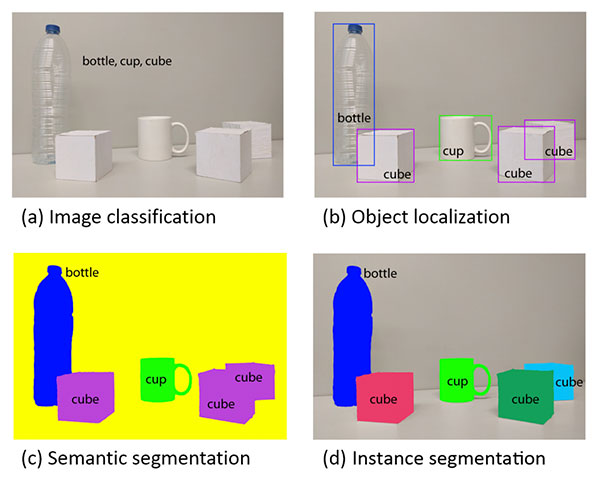
\includegraphics[width=0.7\linewidth]{images/detection/types-of-img-analysis}
	\caption{Similar problems respect to object localization/detection.}
	\label{fig:imgAnalysisType}
\end{figure}



\section{State of the art algorithms}
Object detection has a lot of applications both in real-time, such as in this thesis, but also in safety-critical scenarios like cars with autonomous driving. This division brings out two different metrics: precision and speed. The ideal detector is both fast and precise, however this algorithm does not exist yet. The methods can be divided into two categories.\\
The solutions mainly focus on speed: YOLO (\Cref{sec:yolo}) and SSD (\Cref{sec:ssd}).\\
Instead, the one mainly focused on precision is R-CNN (\Cref{sec:r-cnn}).


\subsection{YOLO (You Only Look Once)} \label{sec:yolo}
YOLO\cite{yolo} was initially designed in 2016. At that time it was the first object detector approach to use a single \textbf{CNN (Convolutional Neural Network)}. Redmon et al. goals were to create an extremely fast detector. An overview of the overall procedure is shown in~\Cref{fig:howItWorks_yolo}, and the architecture appears in~\Cref{fig:architecture_ssdVSyolo}.\\
The image shows a two step procedure, but these steps are solved in parallel. This is the core idea of the paper. A single CNN can be highly optimized.\\
The YOLO procedure works as follows\footnote{The original presentation of YOLO by Redmon at CVPR 2016 conference can be found \href{https://www.youtube.com/watch?v=NM6lrxy0bxs}{here}.}:
\begin{itemize}
	\item Preprocess: the image is resized to fit the standard input dimension of the CNN.
	\item Left image: the picture it is divided into a grid of CxC cells.
	\item Top image: each cell suggests some bounding boxes centred on it, that can match elements in the background. To each box is associated a value describing the probability that it contains one of the elements of the image.\\
	At most one detection per box can be selected as correct. This relies on the assumption that two correct bounding boxes cannot share the centre. This is both an efficient idea but also a big limitation. Too small elements, close to each other, cannot be both detected.
	\item Bottom image: each cell has an associated probability regarding a label that represents the class that can be found in that cell if an element exists in it.\\
	I.e. the cyan cells means: "if there is something here, it will belong to class 'DOG' ".
	\item Right image: the two partial elaborations are merged. The most likely bounding boxes are chosen and classes are associated to them according to the value for each cell in the probability map.
\end{itemize}
That was the first YOLO version, in this thesis is used the third\cite{yoloV3}. Mainly, the changes were about recognition of a wider set of classes and small implementing details to improve the overall precision of the algorithm.\\
\\
The output of the CNN is generated extremely fast and it is accurate however has a big problem. Often if two classes have similar probabilities or the shape of the element is not perfect YOLO might propose more than one bounding box for each element. That is the case of~\Cref{fig:sub_noNMS_yolo} where the truck is classified both as "truck" and as "car". The same happens to the person that has been seen twice.\\
To solve this, it is necessary to apply a new technique: Non-Maximum Suppression.

\begin{figure}[!h]
	\centering
	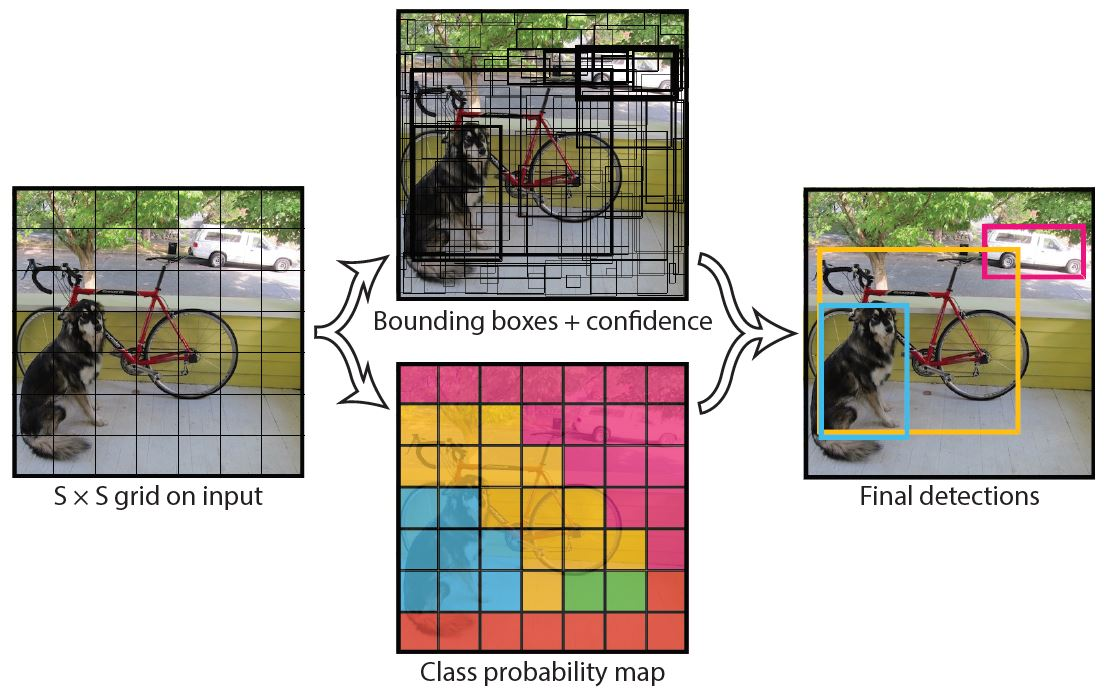
\includegraphics[width=0.8\linewidth]{images/detection/howItWorks_yolo}
	\captionsetup{margin=0.5cm}
	\caption[The steps of the YOLO algorithm.]{The YOLO image elaboration based on bounding box proposal and class probability map.}
	\label{fig:howItWorks_yolo}
\end{figure}

\subsubsection*{NMS (Non-Maximum Suppression)}
This technique\cite{nms} is a post-processing that works on the bounding boxes suggested, as output, from YOLO or other detectors. NMS does not consider the source image. The goal of this procedure is to refine the bounding boxes proposed and to choose which subset of them is better to fit the final image prediction. Two examples of applications are shown in~\Cref{fig:nms}.\\
The main flow of the algorithm is as follows:
\begin{itemize}
	\item The input is a list of all the boxes generated for a single image. Associated to each one there is its probability.
	\item The boxes are sorted in decreasing order according to the probability associated.
	\item Then, each box is accepted or rejected according to the \textbf{IoU (Intersection Over Union)}. That is the percentage of overlapping area with an already accepted box.
	\begin{itemize}
		\item If the IoU is above a certain threshold, meaning that the two boxes overlap too much, the one with the lowest probability is discarded.
		\item If that is not the case, the box is accepted as a new prediction.
	\end{itemize}
\end{itemize}
The input in~\Cref{fig:sub_noNMS}, is processed and only one box is accepted (\Cref{fig:sub_withNMS}) because the IoU is very high. Instead, in~\Cref{fig:sub_noNMS_yolo}, two boxes are removed respectively from two other separated boxes (\Cref{fig:sub_withNMS_yolo}) because two different subjects are involved.

\begin{figure}[!h]
	\centering
	\begin{subfigure}{.13\linewidth}
		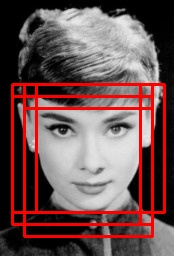
\includegraphics[width=1\linewidth]{images/detection/img1_noNMS}
		\caption{Overlap bounding boxes }
		\label{fig:sub_noNMS}
	\end{subfigure}
	\begin{subfigure}{.13\linewidth}
		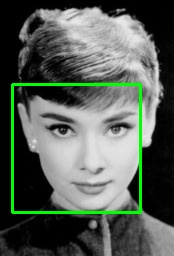
\includegraphics[width=1\linewidth]{images/detection/img1_withNMS}
		\caption{Refined bounding box}
		\label{fig:sub_withNMS}
	\end{subfigure}
	\begin{subfigure}{.35\linewidth}
		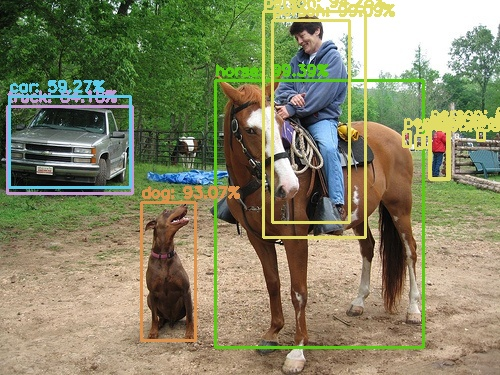
\includegraphics[width=1\linewidth]{images/detection/ex2_yolo_noNMS}
		\captionsetup{margin=0.3cm}
		\caption{YOLO generated bounding boxes}
		\label{fig:sub_noNMS_yolo}
	\end{subfigure}
	\begin{subfigure}{.35\linewidth}
		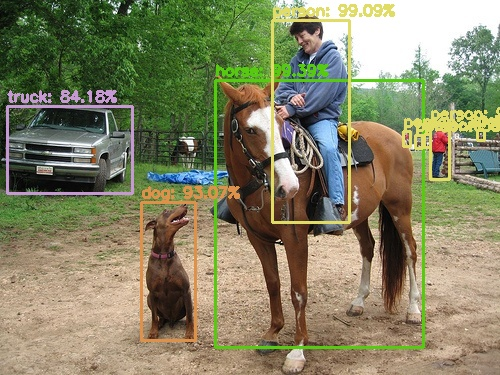
\includegraphics[width=1\linewidth]{images/detection/ex2_yolo}
		\captionsetup{margin=0.3cm}
		\caption{Apply NMS to refine the YOLO's output}
		\label{fig:sub_withNMS_yolo}
	\end{subfigure}
	\captionsetup{margin=0.5cm}
	\caption[Examples of application of NMS post-processing.]{Two scenarios of application of Non-maximum suppression algorithm. First: choose which of the 6 manual generated bounding boxes, on Audrey Hepburn's face, should be considered the correct one. Second: refinement of the YOLO prediction output, by removing the "car" and "person" prediction.}
	\label{fig:nms}
\end{figure}


\subsection{SSD (Single Shot Multibox detector)} \label{sec:ssd}
The principal competitor of YOLO is SSD\cite{ssd}. Both are based on the same principle: the use of a single Convolutional Neural Network to propose bounding boxes and associate them to classes. The CNN is optimized as much as possible to improve the speed performance and eventually even the accuracy.\\
The difference relies on how the two algorithms deal with the bounding boxes suggestion. YOLO for each cell of the grid chooses a couple of options and at most one can be chosen.\\
On the other hand, SSD works as follows (\Cref{fig:howItWorks_ssd}):
\begin{itemize}
	\item The image is divided into a grid of CxC cells, called \textbf{feature map}.
	\item Each cell can propose a set of default boxes that has a size measured in cells (i.e. 3 cells high and 2 wide).
	\item The process is repeated many times varying the value of C: the \textbf{granularity of the grid}. This guarantees that the algorithm is scale-independent matching both, big and small, subjects.\\
	In~\Cref{fig:architecture_ssdVSyolo} is shown how the convolution layers blocks are matched together only at the end.
	\item All the suggestions are merged together to produce the final proposals.
	\item SSD internally performs NMS to remove unnecessary detections.
\end{itemize}

\begin{figure}[!h]
	\centering
	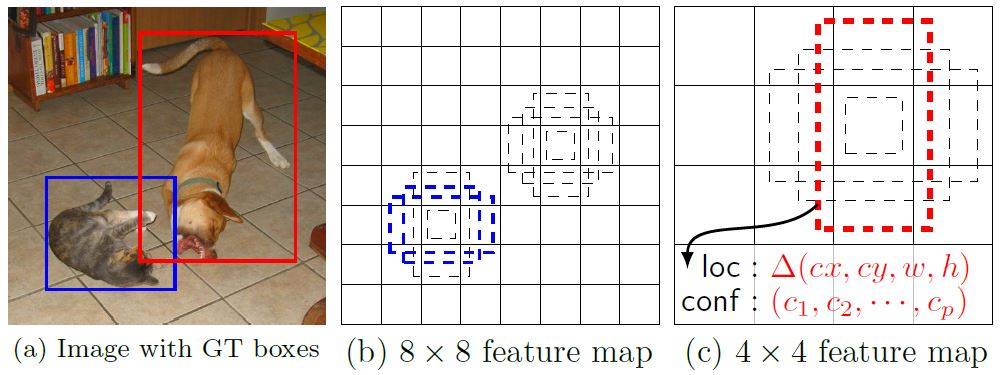
\includegraphics[width=0.8\linewidth]{images/detection/howItWorks_ssd}
	\captionsetup{margin=0.5cm}
	\caption[The steps of the SSD algorithm.]{The SSD image processing and how the bounding box proposal is elaborated.}
	\label{fig:howItWorks_ssd}
\end{figure}
\begin{figure}[!h]
	\centering
	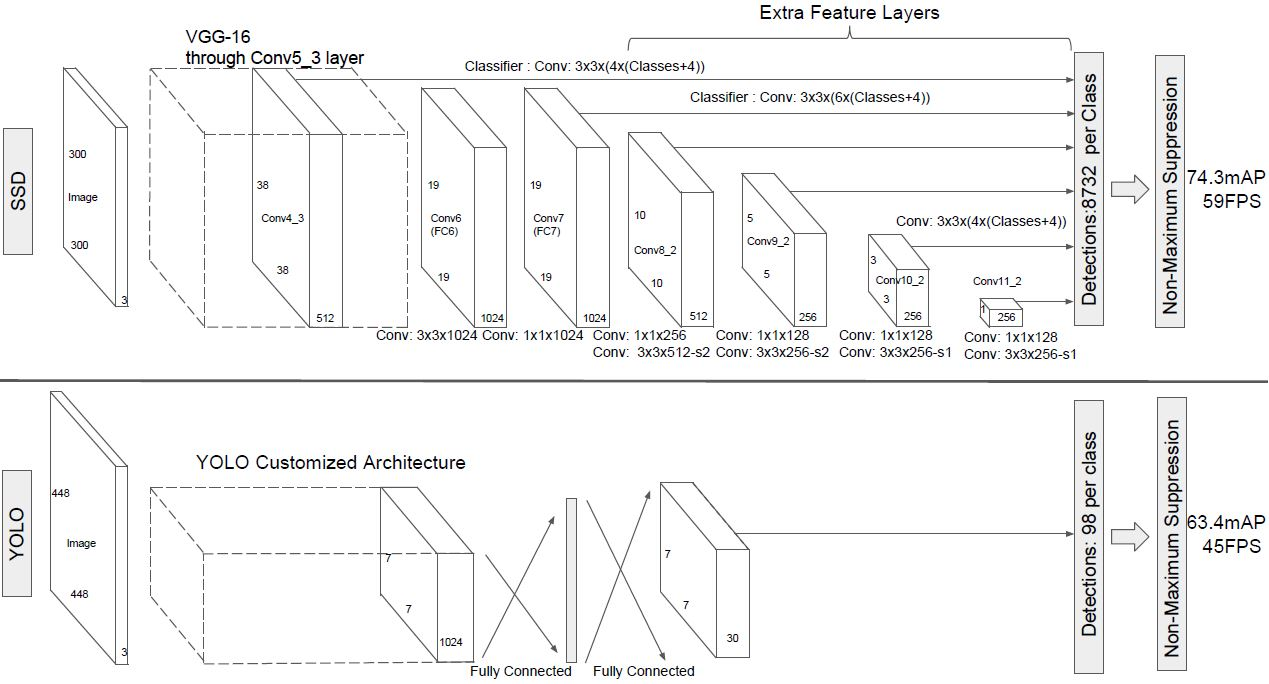
\includegraphics[width=1\linewidth]{images/detection/architecture_ssdVSyolo}
	\captionsetup{margin=0.5cm}
	\caption[Comparison of the architectures of SSD and YOLO.]{A comparison of architectures between SSD and YOLO which is designed as a compact block. Instead, SSD is modular, it is divided into convolution layers of different scales, combined at the end, to make the algorithm scale-independent.}
	\label{fig:architecture_ssdVSyolo}
\end{figure}


\subsubsection*{MobileNet}
The implementation of the project does not use a traditional version of SSD, but a lighter one. This model is a combination of SSD and mobileNet\cite{mobilenet}.\\
MobileNet is a methodology that approaches Convolutional Neural Networks to transform the architecture structure to build a much lighter version of the model. The concept was first ideated to allow low power devices, such as smartphones, to run computational expensive algorithms based on CNN.\\
The principle is to replace each standard convolution (\Cref{fig:sub_architecture_mobileNet1}) with a \textbf{Depthwise separable filter}. A standard convolution works on a grid of DxD pixels and for each one produces output features of depth M. This operation can be repeated N times for each source feature.\\
The operation is broken into two other simpler convolutions:
\begin{itemize}
	\item \textbf{Depthwise convolutional filters} (\Cref{fig:sub_architecture_mobileNet2}): produces only one feature output at a time, repeated M times for each DxD grid.
	\item \textbf{Pointwise convolution filters} (\Cref{fig:sub_architecture_mobileNet3}): extends the output feature of the depthwise filter to N output features.
\end{itemize}
The original paper demonstrates how these two operations stacked in a row, can produce results close to the correct ones.\\
The computational cost determined by the number of parameters, used by depthwise and pointwise filters, can be further reduced by randomly removing a percentage of these parameters. According to the portion of parameters removed (25\%, 50\%, 75\%), the algorithm precision is affected.

\begin{figure}[!h]
	\centering
	\begin{subfigure}{0.32\textwidth}
		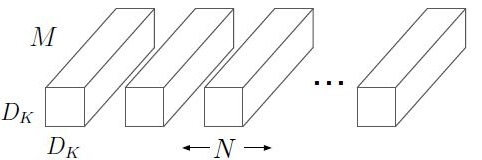
\includegraphics[width=\linewidth]{images/detection/architecture_mobileNet1}
		\caption{Standard convolution filters}
		\label{fig:sub_architecture_mobileNet1}
	\end{subfigure}
	\begin{subfigure}{0.32\textwidth}
		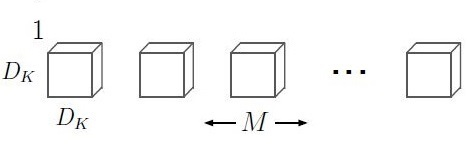
\includegraphics[width=\linewidth]{images/detection/architecture_mobileNet2}
		\caption{Depthwise convolutional filters}
		\label{fig:sub_architecture_mobileNet2}
	\end{subfigure}
	\begin{subfigure}{0.32\textwidth}
		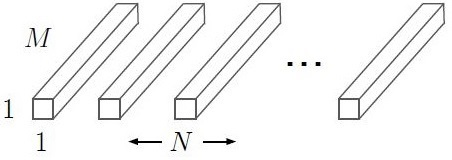
\includegraphics[width=\linewidth]{images/detection/architecture_mobileNet3}
		\caption{1x1 convolutional filters called Pointwise convolution filters}
		\label{fig:sub_architecture_mobileNet3}
	\end{subfigure}
	\captionsetup{margin=0.5cm}
	\caption[The schemes of convolutions introduced by mobileNet.]{The novelty of mobileNet is that it converts a traditional convolution (A), into a combination of two lighter convolutions (B-C), that produce almost the same output.}
	\label{fig:architecture_mobileNet}
\end{figure}


\subsection{R-CNN (Region-based Convolutional Neural Networks)} \label{sec:r-cnn}
\textbf{R-CNN}\cite{r-cnn} was the first invented method of the three in this section. Differently from YOLO and SSD, it is mainly focused on performing detections with high precision, despite the processing time.\\
This algorithm is a two step object detector. The workflow, shown in~\Cref{fig:howItWorks_rcnn}, works as follows:
\begin{enumerate}
	\item A region proposal algorithm is executed on the input image and it produces 2000 bounding boxes.
	\item Each of these proposals are elaborated independently. \\
	For each box, an image classifier, based on CNN, produces features from the image and then predicts which classes they might contain.\\
	Any kind of image classifier can be used for this task resulting in an algorithm that can be easily adapted with new networks.
\end{enumerate}
The main problem is that overlapping proposals are elaborated independently. The result is that feature extraction is performed on the same area of the image multiple times. These have been solved with a second version of the algorithm, called \textbf{Fast-R-CNN}\cite{fast-r-cnn}. The feature extraction for the full image is performed before the image classification that now works on an already generated image of features.\\
An incremental improvement, comes from the third version: \textbf{Faster-R-CNN}\cite{faster-r-cnn}. It performs the feature extraction as the first step and based on it the bounding boxes are proposed with \textbf{RPN (Region Proposal Network)}. The modified structure allows ad hoc optimizations to improve the low processing time.

\begin{figure}[!h]
	\centering
	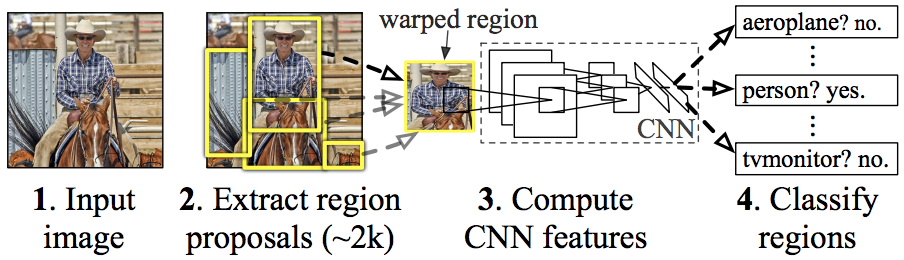
\includegraphics[width=0.8\linewidth]{images/detection/howItWorks_rcnn}
	\caption{The 2-step elaboration of R-CNN model on a sample image.}
	\label{fig:howItWorks_rcnn}
\end{figure}



\section{Other famous algorithms}
\subsection{Mask R-CNN} \label{sec:mask-r-cnn}
A variation of R-CNN that aims to solve the instance segmentation task (\Cref{fig:imgAnalysisType}) is Mask R-CNN\cite{mask-r-cnn}.\\
Mask R-CNN is built on top of two technologies:
\begin{itemize}
	\item Faster R-CNN used as an object detector.
	\item \textbf{FCN (Fully Convolutional Network)}\cite{fcn} that performs semantic segmentation.
\end{itemize}
For each bounding box, it is known the class, then FCN computes the segmentation of that class. All the shapes of elements in the image are then merged together to build the instance segmentation result. An application of this algorithm is shown in~\Cref{fig:ex2_maskRCNN}.

\begin{figure}[!h]
	\centering
	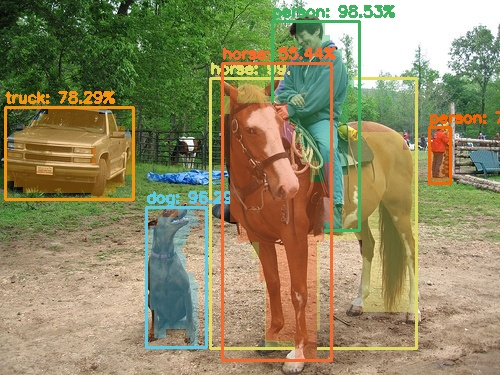
\includegraphics[width=0.7\linewidth]{images/detection/ex2_maskRCNN}
	\caption{Instance segmentation of an image using mask R-CNN.}
	\label{fig:ex2_maskRCNN}
\end{figure}


\subsection{Open Pose} \label{sec:openpose}
Firstly designed in 2017 OpenPose\cite{openpose-PAF} aims at processing an image and recognising the position of the people in it. The position is the skeleton of a person, it is the interconnection of limbs that link 15 points on the human body.\\
This algorithm opens al lot of possibilities because until then estimating the body position was achieved with 3D cameras, extremely expensive hardware that now can be easily substituted. Recently, OpenPose has been improved in terms of speed, to process frames in a video with \textbf{STAF (Spatio-Temporal Affinity Field)}\cite{openpose-STAF}, and it is also been extended to understand the 3D human position.\\
An overview of the overall procedure of the algorithm is shown in~\Cref{fig:howItWorks_openpose}, instead some output examples are shown in~\Cref{fig:ex_openpose}.\\
The OpenPose procedure works as follows\footnote{The original demo of OpenPose by Zhe Cao at CVPR 2017 conference can be found \href{https://www.youtube.com/watch?v=pW6nZXeWlGM}{here}.}:
\begin{enumerate}[a)]
	\item Preprocessing: the input image is reshaped to match the requirements of the two-branch CNN.
	\item Part Confidence Maps: the first branch of the CNN process the image to extract the location of the 15 body parts.\\
	Each body part (i.e. left shoulder, left knee, right wrist...) is detected by an ad hoc filter. These filters do not process one person at a time but the entire image simultaneously. The result is that a filter recognises all the visible right elbows in the image. This is extremely important because, by doing this, the algorithm process speed is independent respect to the number of people in the image.
	\item Part affinity fields: the second branch of the CNN process the image to recognise the limbs that can connect all the body points found so far.
	\item Bipartite matching: has the goal to match all the elements found to reconstruct the skeleton of the entire person.\\
	This reconstruction is a greedy approach mainly based on geometry that wants to minimize the distance of two parts that must be connected.
	\item Parsing results: the output image is assembled with the full-body poses for all people in the image.
\end{enumerate}
It is important to note that OpenPose is a bottom-up approach. The algorithm has no knowledge about the positioning of people in the image, it only tries to reconstruct the skeleton from small sections of the body.

\begin{figure}[!h]
	\centering
	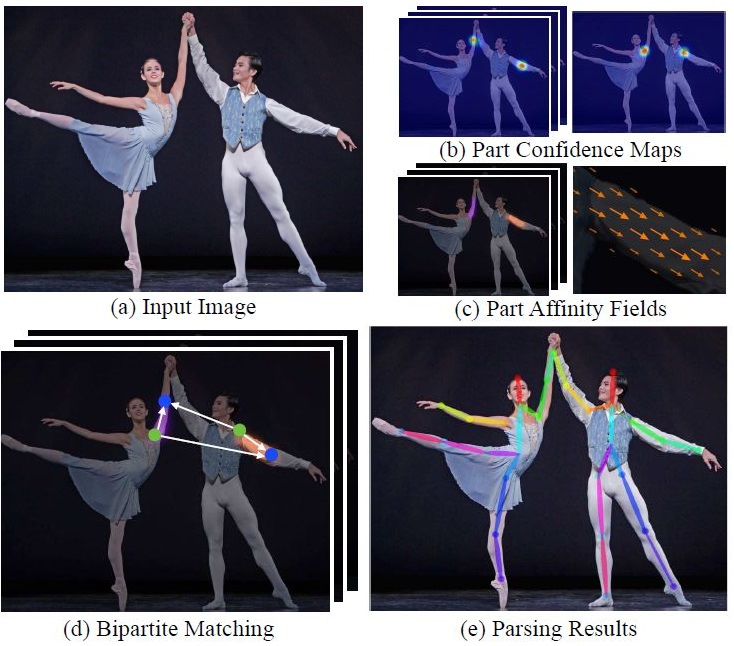
\includegraphics[width=0.8\linewidth]{images/detection/howItWorks_openpose_2line}
	\captionsetup{margin=0.5cm}
	\caption[The steps of the OpenPose algorithm.]{The elaboration of the OpenPose algorithm to recognise the skeleton of the two dancers in the image.}
	\label{fig:howItWorks_openpose}
\end{figure}
\begin{figure}[!h]
	\centering
	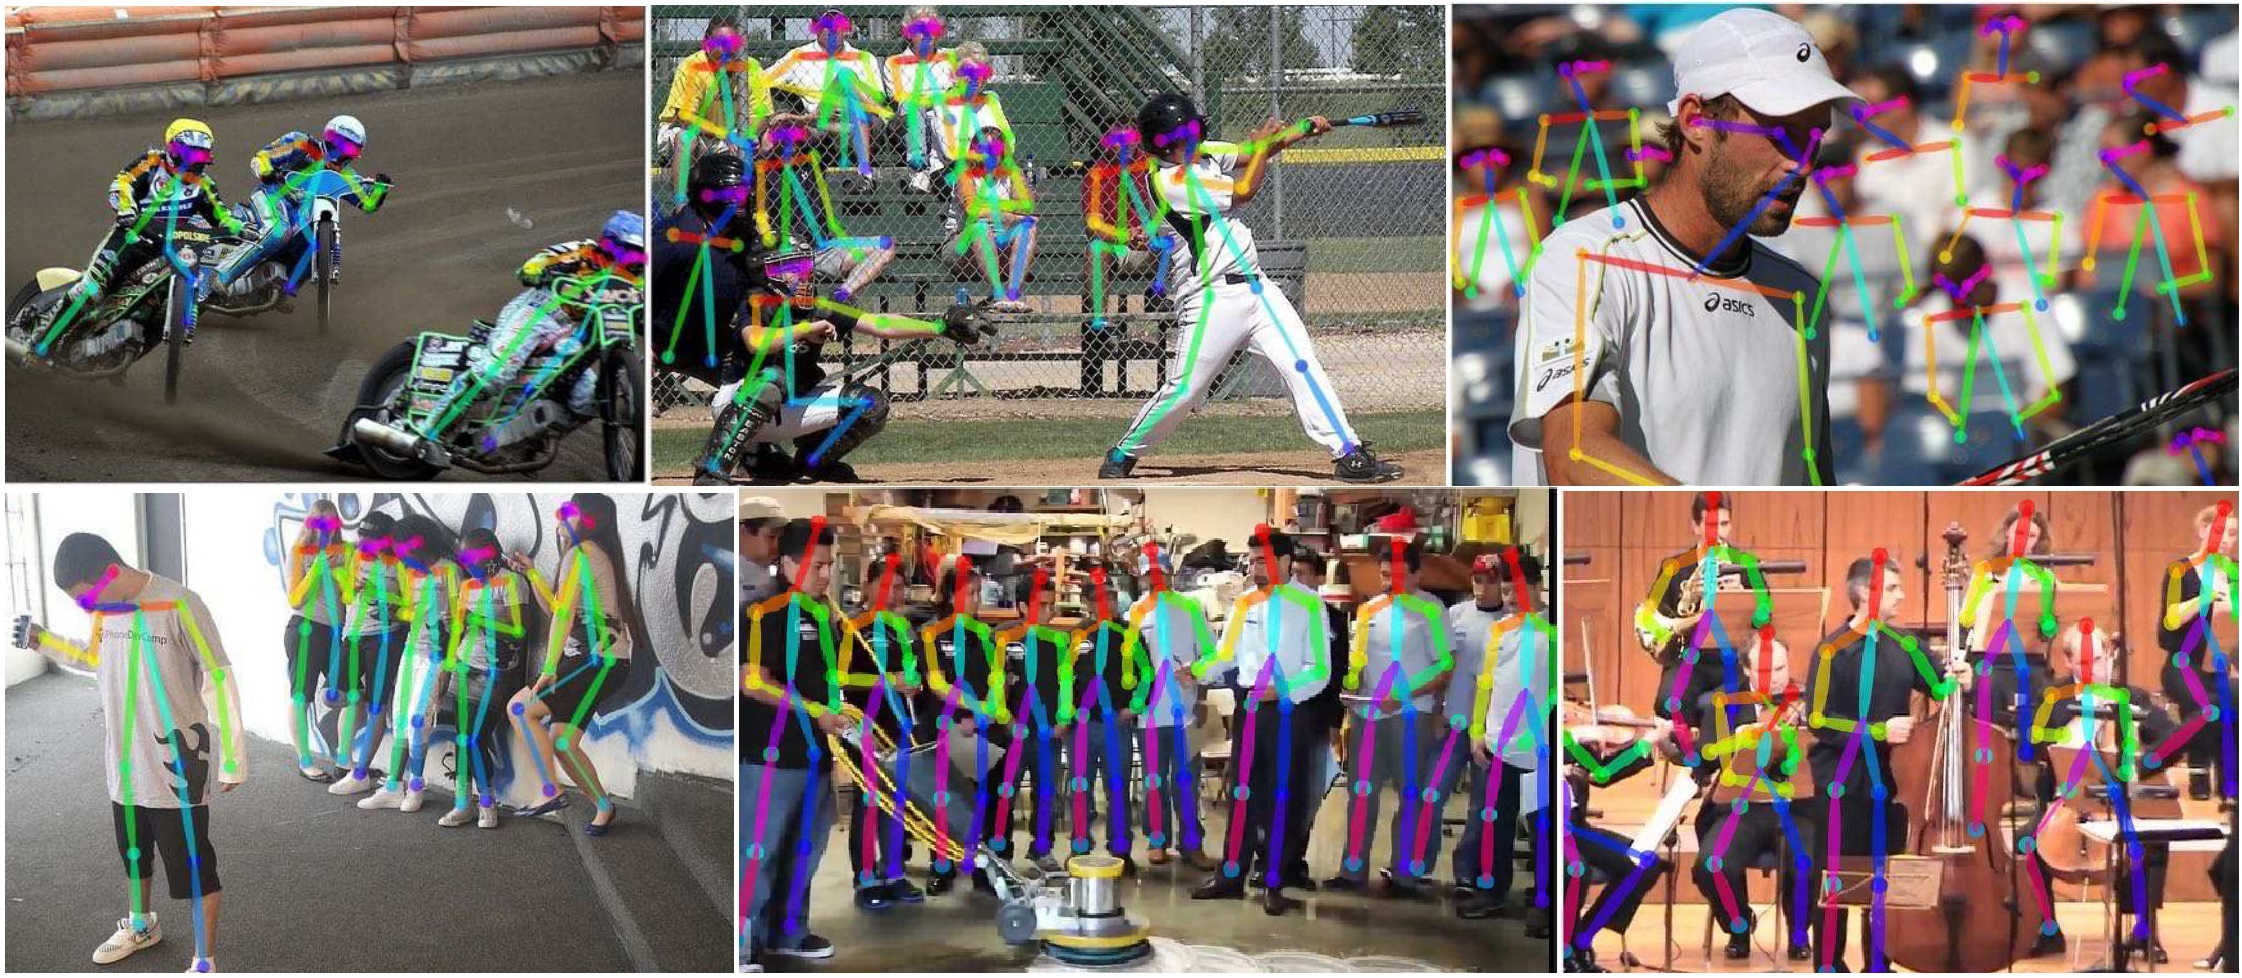
\includegraphics[width=1\linewidth]{images/detection/ex_openpose_2line}
	\captionsetup{margin=0.5cm}
	\caption[Examples of application of OpenPose.]{Some examples, taken from the original paper, on how OpenPose works.}
	\label{fig:ex_openpose}
\end{figure}



\section{Overview of the algorithms}
The algorithms presented in this chapter represent the state of the art methods for their field of application.\\
All those methods can be used to achieve the long-term tracking that is the goal of this thesis, but the different information generated should be used to solve the problem with different approaches. We have chosen to use the methods that perform only the detection task. This results on one hand into general information as output, and on the other hand into a very high processing speed that is fundamental for real-time application.

\subsubsection*{Performances comparison}
A comparison of the speed, measured as \textbf{FPS (Frames Per Second)}, and of the precision, measured as \textbf{mAP (mean Average Precision)}, is shown in~\Cref{tab:detectionPerformances}. The data are based on the Pascal VOC 2007 dataset\cite{pascal-voc-2007} and come from multiple papers\cite{yolo}\cite{yoloV2}.\\
The measures do not show YOLOv3 because compared to the other methods it is more recent and a fair comparison does not exist. Instead, for Mask R-CNN and OpenPose, only the frame rate is shown because the mAP can be computed. However it is completely irrelevant respect to the other presented in the table. These two algorithms perform different tasks hence the precision of the result cannot be compared.\\
By looking at the data, it clearly appears that the single-stage algorithms (SSD and YOLO) are much faster respect to the two-stage methods (R-CNN), in fact, they run around 5-10 times faster than R-CNN. Instead, the precision of the three detectors is almost the same. For these reasons, we have chosen to use in this project the last version of YOLO and a lighter version of SSD: mobileNet-SSD. This idea pays a few percentage points in term of mAP but implements the CNN with fewer parameters, results in a low power consumption method. This aspect is important because the robots do not mount top quality hardware, therefore the light version of SSD can be executed more easily.

\subsubsection*{Output visualization}
To visually show the potentialities of these algorithms we have applied all of them on the same picture. This elaboration is presented in~\Cref{fig:ex_detectionAlgorithms}. Independently from the task that they solve, it appears evident that all of them recognise the 5 people in the foreground, but there are some differences:
\begin{itemize}
	\item SSD has troubles with the player on the left. In fact, the percentage associated with him is only a 32\%.
	\item YOLO is able to detect even a sixth person in the background that none of the others have seen.
	\item YOLO is trained to recognise a wide variety of objects respect to the other detectors, in fact, it is able to recognise even the "sports ball".\\
	Even SSD is adaptable and can be trained to recognise the ball. However the big advantage of the second version of YOLO (also called \textbf{YOLO9000}), is that it was integrated with the \textbf{Wordnet graph}\cite{wordnet} to be scalable in terms of the number of classes recognised. The result is a detector that is able to recognise up to 9000 different classes.
	\item Mask R-CNN is, in this example, the most accurate algorithm. It recognises four people with a precision of 99\% and the last one with 92\%. 
	\item OpenPose, by estimating the body parts, can even understand the orientation of the people in the soccer field. This big advantage can be used to understand where these people will move in the frame after this one.
\end{itemize}
Considering these reasons, it is evident that discarding OpenPose and Mask R-CNN, in favour of SSD and YOLO, is only a choice for this project. All these algorithms have potentiality that can be used to create a good object tracker.

\begin{table}[!h]
	\centering
	\begin{tabular}{|c|c|c|c|c|c|c|c|c|}
		\hline
		Pascal VOC 2007 & \multicolumn{2}{c|}{YOLO} &     & \multicolumn{4}{c|}{R-CNN}   &          \\ \hline
		Algorithm       & v1          & v2          & SSD & R-CNN & Fast & Faster & Mask & OpenPose \\ \hline
		FPS             & 45          & \textbf{67}          & 46  & 0.05  & 0.5  & 7      & 7    & 10       \\ \hline
		mAP             & 66          & \underline{\textbf{76}}          & \underline{74}  & 53    & 70   & \underline{73}     & X    & X        \\ \hline
	\end{tabular}
	\captionsetup{margin=0.5cm}
	\caption[Comparison of mAP and FPS for the object detector algorithms.]{Overview of the performances of the algorithms presented. The evaluation is based on the mAP and the processing speed. In bold the best scores and underlined the mAP of the three states of the art detectors.}
	\label{tab:detectionPerformances}
\end{table}
\begin{figure}[!h]
	\centering
	\begin{subfigure}{.45\linewidth}
		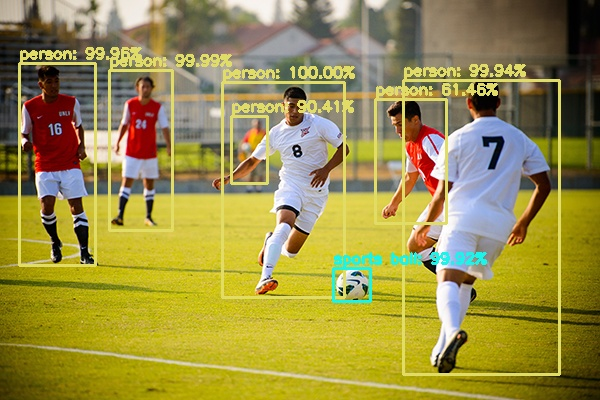
\includegraphics[width=\linewidth]{images/detection/ex3_yolo}
		\caption{YOLOv2: detection}
	\end{subfigure}
	\begin{subfigure}{.45\linewidth}
		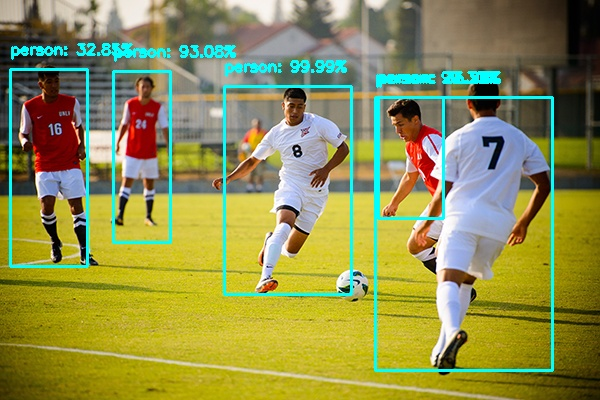
\includegraphics[width=\linewidth]{images/detection/ex3_ssd}
		\caption{SSD: detection}
	\end{subfigure}
	\begin{subfigure}{.45\linewidth}
		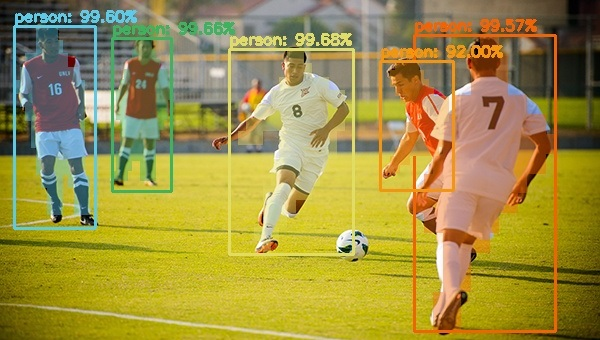
\includegraphics[width=\linewidth]{images/detection/ex3_mask-rcnn}
		\caption{Mask R-CNN: instance segmentation}
	\end{subfigure}
	\begin{subfigure}{.45\linewidth}
		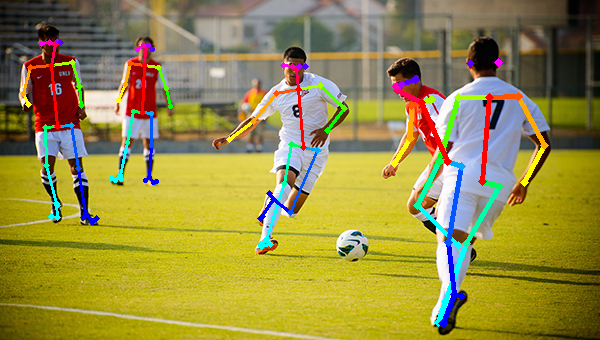
\includegraphics[width=\linewidth]{images/detection/ex3_openpose}
		\caption{OpenPose: human pose estimation}
	\end{subfigure}
	\captionsetup{margin=0.5cm}
	\caption[YOLO, SSD, Mask R-CNN and OpenPose applied on the same image.]{An example of application of the four main algorithms, based on the same sample image.}
	\label{fig:ex_detectionAlgorithms}
\end{figure}






 	\clearpage
      \chapter{Object Tracking} \label{cha:tracking}
This chapter is focused on a few methods that solve the traditional task of object tracking. For each algorithm the potentiality is shown and the advantages, compared to other methods, will be discussed. In addition, an overview of similar problems is given in~\Cref{sec:tracking-conditions}.



\section{Task definition} \label{sec:tracking-definition}
Object tracking is a challenge that, differently from the detection, does not work with images but deal with videos. A video is technically defined as a sequence of images, called \textbf{frames}, combined together at a certain frame rate. Typically this rate is 15, 30 or 60 FPS (Frames Per Second).\\
The interconnection of the frames of videos is used from the object tracker algorithms to create knowledge, based on the previously analysed images, by storing information. An object detector elaborates a picture at a time, each one independently from the other. There is no connection among images of the same database. Instead, a tracker process images one at a time but it uses the knowledge, of the previously analysed frames, to understand the current incoming image.\\
The task baseline is defined as:
\begin{tcolorbox}
	\begin{center}
		\textit{\textbf{The traditional tracking challenge} consists of tracking a single well-defined subject over a short video clip, no matter if it is a person, an animal or an inanimate object. The target of the tracking clearly fully appears into all the frames of the sequence.}
	\end{center}
\end{tcolorbox}


\subsection{Interface}
Structure of the tracking algorithms interface:
\begin{itemize}
	\item One input value is composed of an image, typically the first frame of a video. In our case of real-time elaboration the image corresponds to the actual view of a webcam connected to the device.
	\item The other input corresponds to the bounding box coordinates of the subject that needs to be tracked. The bounding box can be manually generated or can be automatically identified with an object detector.
	\item All future steps get as input a new frame. The task is to understand, in this new image, where is located the subject defined by the initial bounding box.\\
	Then, if all these elaborated images and the generated bounding boxes, are combined together, the result is a video. The initial subject of the video while moving is always centred into a rectangle that follows it across the entire \textbf{FoV (Field of View)} of the camera.
\end{itemize}


\subsection{Subject of the tracking}
It is important to note that the task is called "\textit{Object tracking}" and not "\textit{Person tracking}" this is because there are no limitations to the subject that needs to be tracked, it does not necessarily need to be a human. A better name for the challenge could be "\textit{Area tracking}" because the algorithms should follow the rectangle of coloured pixels that was located in the initial bounding box. No assumption can be done of which type of subject exists inside the bounding box.\\
Generally, these methods work if the initial position is centred around an object that moves consistently in the space and does not change aspect. Some examples that could break these methods are:
\begin{itemize}
	\item The initial bounding box contains two or more objects that move independently from each other. The algorithm will recognise one of the two as the main subject and will track it over the video and lose the other one. \\
	This is a problem if accidentally the bounding box contains something that is "more important" than the "\textit{real subject}". It can also be an advantage that allows to easily discard the background that is an "\textit{object}" itself.\\
	Since two independent objects move differently in the space compared to a single unique object, tracking them can easily create unexpected errors due to inconsistent movements.
	\item The subject changes aspect too rapidly due to different luminosity in the environment, or elaborated video sequences that are not "\textit{natural}". This last possibility often breaks methods designed for real situations, so it is not a problem only in this case. Instead, the change of luminosity often occurs but a solution can be achieved with frame pre-processing, such as the standardization of the luminosity of the image to always process a figure with the same luminosity.
\end{itemize}


\subsection{Deal with special conditions}\label{sec:tracking-conditions}
The tracking task can be seen as a set of problems. This is because there are a lot of conditions that can modify the scenario where the algorithms should work. By modifying the type of difficulties in the videos some methods may fail while others may not.\\
The goal of this thesis is to build a "person tracker", that should work under certain conditions. The problem is that the combination of a lot of requirements makes the problem harder.\\
Despite the time spent for a programmer to ideate, implement and test a solution there is a trade-off to consider. Solving a hard task requires a more computational complex solution compared to solving a similar easier task. This complexity influences the performances of the proposed algorithm. To conclude, it is important to understand which are the requirements of the problem that we are dealing with, in order to choose the algorithm that it is better to use, to solve the task and to perform it fast.\\
\\
Below are listed a set of requirements that make the baseline harder (definition is in~\Cref{sec:tracking-definition}):
\begin{itemize}
	\item \textbf{Changes of 2D shape}: the target due to movements might change its ratio, aspect, and shape. We are interested in what the camera sees of the subject (2D  space) and not the effective actual condition of the subject (3D space).
	\begin{itemize}
		\item \underline{Partial occlusion} (\Cref{fig:challenge_partialOcclusion}): it may happen that during the video, part of the subject is occluded, by an object. If this happens the algorithms must be designed to be robust and to localize the target even with a small section of it.\\
		The bounding box generated may contain only the visible part of the subject but it may also happen that an estimation of the entire subject is done and the bounding box contains both the visible and the estimated missing area of the target.
		\item \underline{Rotations and deformations} (\Cref{fig:challenge_deformation}): the object tracked while moving can rotate and show to the camera a different side, or if it is deformable, change the shape (i.e. a person walking change the shape continuously). This might influence even colours.
	\end{itemize}
	
	\item \textbf{Total occlusion} (\Cref{fig:challenge_totalOcclusion}): the subject completely disappears behind an object or out of the camera field of view.
	\begin{itemize}
		\item \underline{Short-time occlusion}: the subject is hidden for a very small number of frames (i.e. 5 or less). This often happens when the subject or an obstacle is moving and the three elements, subject, object and camera, are aligned. These very short occlusions may be solved using a little memory that stores the subject information for the last few frames (i.e. 10).
		\item \underline{Long-time  occlusion}: the occlusion lasts for a bigger number of frames, even seconds. Often it occurs when the subject exits the field of view of the camera and does not enter it again for a while. It can also happen if the subject is behind a big obstacle such as a vehicle or a wall.\\
		It is harder to solve compared to the previous scenario, because the solution requires a long term memory associated with a recognition procedure to understand when the subject is visible back again.
	\end{itemize}

	\item \textbf{Fast-moving object}: the subject shifts for a big portion of the picture from the old position to the new one in a single frame. Meaning that there was a big 2D movement. This could happen because the subject is effectively moving fast, or because it is close to the camera and even a small movement looks big.
	\begin{itemize}
		\item \underline{Blurred subject} (\Cref{fig:challenge_blurred}): due to its movement the subject is blurred and this heavily changes its aspect. The modified elements are the shape and the colours that are somehow faded. In addition, especially for humans, moving fast can make parts of the body such as arms or legs disappear.
		\item \underline{Proximity assumption} (\Cref{fig:challenge_proximity}): a lot of trackers are based on the assumption that the subject moves around only a little bit. If it moves fast this principle is broken.\\
		After knowing the exact location of the subject on the previous frame starts the estimation on the following one.\\
		At this point there are two things to focus on:
		\begin{itemize}[\ding{228}] %method to insert custom symbol in itemize (\ding(228) = the full >)
			\item If the subject does not move is probable that the prediction will place the target in the exact same position as before. Instead, if it moves the probability that the tracked object will be located close to the previously known position is higher than to be located far away. Specifically, the likelihood can be seen as a \textbf{Multivariate Normal Distribution} centred at the previous position and stretched towards the direction where the subject is moving (\Cref{fig:challenge_multivariate}).
			\item If multiple similar objects exist in the frame and the tracking is following one of them, it is probable to lose it. This happen with a fast movement that generates an unpredictable big shift, and the target moves far away from the previous position while the tracker recognise its subject into a similar object. From now on, the tracking is broken because it follows the wrong physical element.
			\item A big shift can also be wrongly interpreted as a total occlusion.
			\item On the other hand, reducing the tolerance to big movement allows the algorithms to only search locally around the last known position resulting in a big improvement of the overall performance.
		\end{itemize}		
	\end{itemize}

	\item \textbf{Low-resolution images} (\Cref{fig:challenge_lowResolution}): as with many other computer vision challenges the resolution of the input image is fundamental. A low number of pixels per frame results into a bounding box (often a small portion of the entire image) of very low resolution. Because of this, recognising the key elements that identify the subject is hard, but also faster and computationally cheaper.

	\item \textbf{Moving background/camera}: working on a fixed camera allows the use of a set of techniques based on background subtraction. The key idea is to get prior knowledge of the background and understand which objects are there, by removing the known part pixel by pixel. A big change of luminosity can make this harder, but still possible.\\
	A camera that rotates always on the same section can be managed as a fixed camera. This can be done by combining all the images along with the rotation as a unified one, creating a \underline{panorama image}.\\
	Instead, a moving camera implying a moving background makes everything harder:
	\begin{itemize}
		\item No background subtraction can be done.
		\item The subject may change aspect even if it does not move.
		\item The occlusion, both partial and total, can occur more easily.
		\item A zoom or rotation of the camera causes a similar effect such as the "fast-moving object".
		\item To estimate the movement speed and direction of the subject it is necessary to know the movement of the camera because one is relative to the other. However, almost always the displacement of the camera in the space is unknown.
	\end{itemize}

	\item \textbf{Real-time}: designing a method to run in real-time requires to focus on the computational capability and respectively to the processing speed. Real-time might vary from 1 to 60 FPS according to the application. To achieve this speed it is often necessary to choose a faster method instead of an accurate one. This reduces the overall precision of the entire designed algorithm.\\

	\item \textbf{Long-term video sequences}: the input frame sequence is longer than a few seconds, up to minutes. Firstly, a long video might easily contain some of the problems listed above. In addition, trying to locate the same subject over and over again without a reinitialization can fail due to the drift problem.\\
	The \textbf{drift problem} consists of an accumulation of small errors along the tracking period. A tracking algorithm refers to the bounding box generated for the previous frame. The subject that should be located again in the new frame is extracted from that bounding box. If the tracking lasts for a small number of frames, the subject may look similar to the original one. Instead, during a long processing the bounding box starts to derive from the original subject. Due to partial occlusion, the box might be reduced. Due to a strong change of luminosity, the bounding box might be misaligned. Due to a fast movement, the box can be linked to the background. By continuing summing up all these little problems the main subject will be recognised as a superfluous element. Therefore the tracker stops to consider it useful and the track fails.\\
	To solve this problem the solution is to re-initialize the tracker often before reaching the limit of the drift. This can be done with different methods such as a \textbf{Kalman filter} or by recognising the main subject with a detection, that is the method presented in this thesis.
	
	\item \textbf{Multiple subjects} (\Cref{fig:challenge_multiple}): if there is more than a subject to follow the naive solution is to apply an object tracker to each of them. Each tracker works independently from the others therefore given $X$ subjects the performances $f$ measured in FPS are reduced to $f/X$.\\
	An efficient solution consists of considering all the tracked subject at the same time with a single algorithm instance.
	
	\item \textbf{Type of the subject} (\Cref{fig:challenge_differentSubject}): the baseline problem does not assume any kind of prior knowledge about which type of subject should be tracked. However sometimes ad hoc solutions are required, which simplify the problem. Frequent choices are people (such in this thesis), animals, vehicles or inanimate objects. For example, if vehicles are chosen the change of shape is not a problem because a car always looks the same.
	
\end{itemize}
\begin{figure}[!h]
	\centering
	\begin{subfigure}[!h]{0.19\textwidth}
		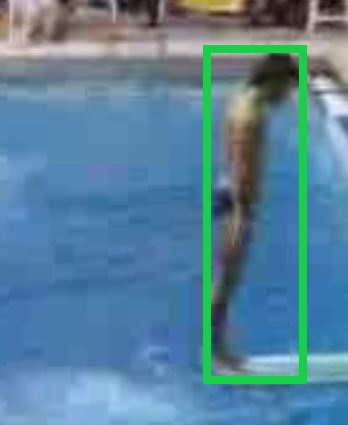
\includegraphics[width=\linewidth]{images/tracking/challenge_lowResolution}
		\caption{Images with low resolution.}
		\label{fig:challenge_lowResolution}
	\end{subfigure}
	\begin{subfigure}[!h]{0.54\textwidth}
		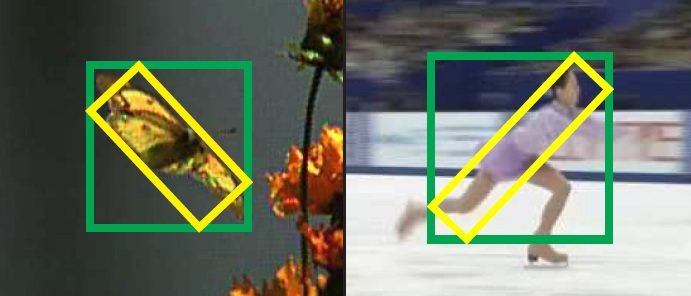
\includegraphics[width=\linewidth]{images/tracking/challenge_deformation}
		\captionsetup{margin=0.5cm}
		\caption{Two subject that can vary their appearance very quickly.}
		\label{fig:challenge_deformation}
	\end{subfigure}
	\begin{subfigure}[!h]{0.24\textwidth}
		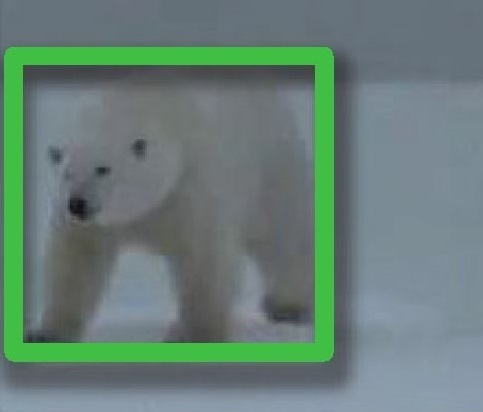
\includegraphics[width=\linewidth]{images/tracking/challenge_differentSubject}
		\caption{Tracking deals with objects, humans, and even animals.}
		\label{fig:challenge_differentSubject}
	\end{subfigure}
	%
	\begin{subfigure}[!h]{0.19\textwidth}
		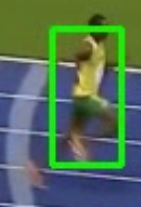
\includegraphics[width=\linewidth]{images/tracking/challenge_blurred}
		\caption{The limbs disappears.}
		\label{fig:challenge_blurred}
	\end{subfigure}
	\begin{subfigure}[!h]{0.49\textwidth}
		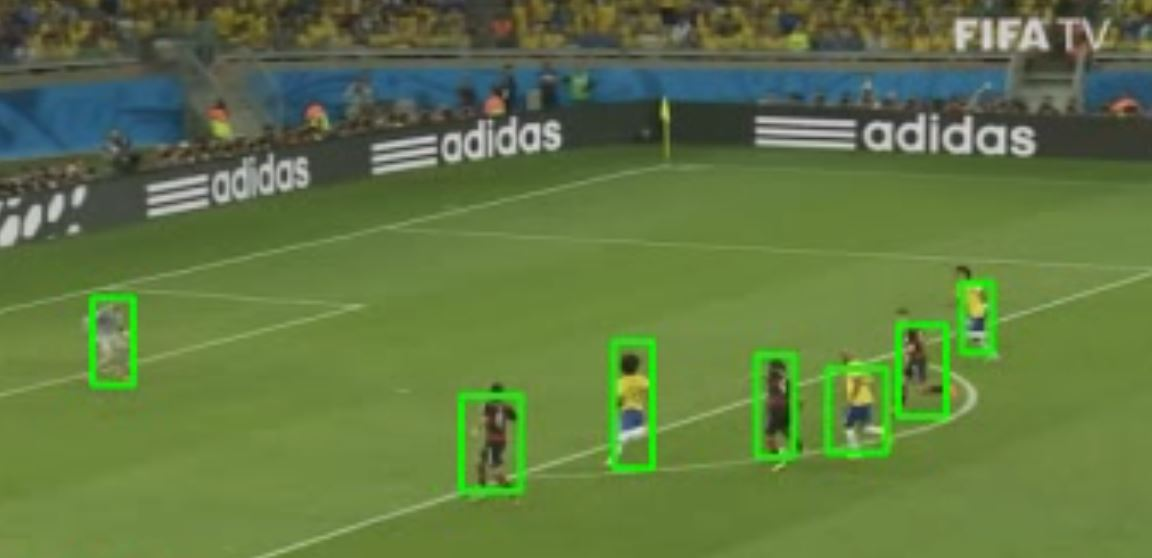
\includegraphics[width=\linewidth]{images/tracking/challenge_multiple}
		\captionsetup{margin=0.5cm}
		\caption{A soccer match action where all the players are tracked.}
		\label{fig:challenge_multiple}
	\end{subfigure}
	\begin{subfigure}[!h]{0.29\textwidth}
		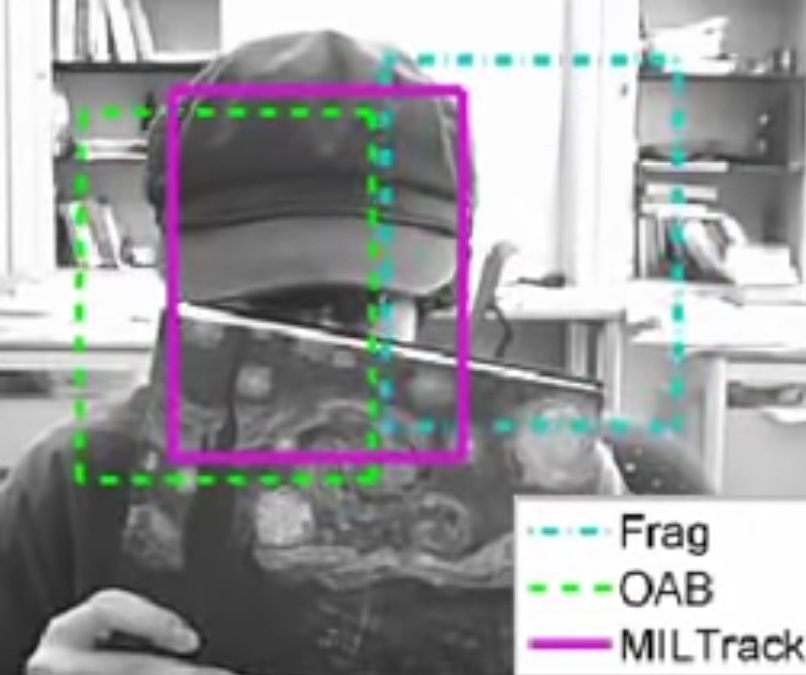
\includegraphics[width=\linewidth]{images/tracking/challenge_partialOcclusion}
		\caption{A face partially hidden by a hat and a book.}
		\label{fig:challenge_partialOcclusion}
	\end{subfigure}
	%
	\begin{subfigure}[!h]{0.49\textwidth}
		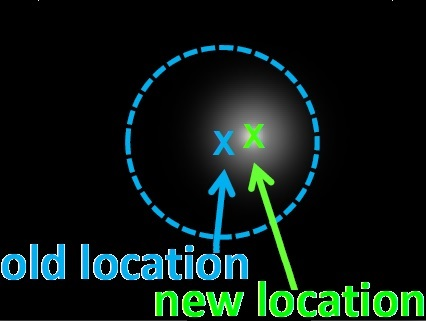
\includegraphics[width=\linewidth]{images/tracking/challenge_proximity}
		\caption{The new location is close to the older one.}
		\label{fig:challenge_proximity}
	\end{subfigure}
	\begin{subfigure}[!h]{0.49\textwidth}
		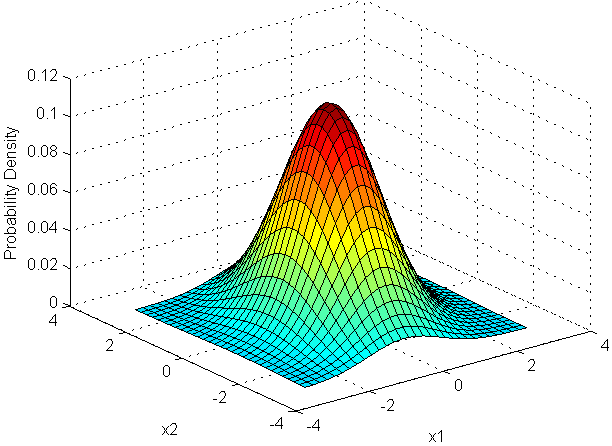
\includegraphics[width=\linewidth]{images/tracking/challenge_multivariate}
		\captionsetup{margin=0.5cm}
		\caption{The probability of where the new location is respect a multivariate normal distribution.}
		\label{fig:challenge_multivariate}
	\end{subfigure}
	%
	\begin{subfigure}[!h]{1\textwidth}
		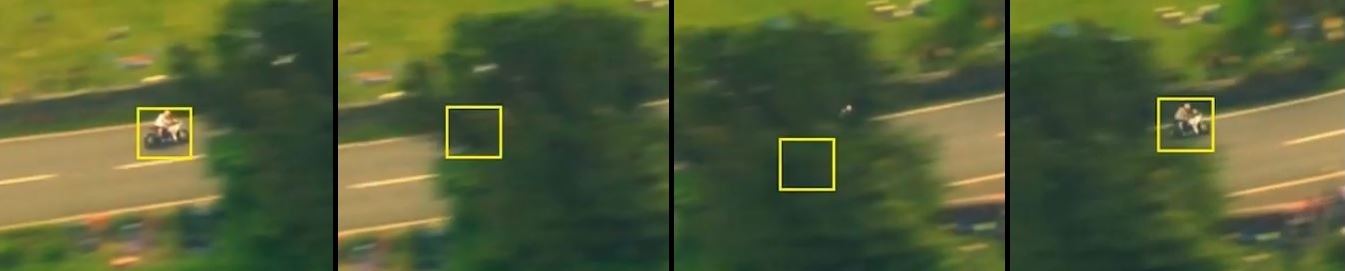
\includegraphics[width=\linewidth]{images/tracking/challenge_totalOcclusion}
		\caption{A motorcycle running on a street, is totally hidden by a tree for multiple frames.}
		\label{fig:challenge_totalOcclusion}
	\end{subfigure}
	\caption{Some visual examples of the tracking challenge conditions.}
	\label{fig:trackingChallenges}
\end{figure}


\subsection{The traditional tracking problem compared to the thesis project} \label{sec:trackingBaseliveVsThesis}
Some of the aspects explained in the previous section are extremely frequent in a lot of videos and databases, hence they are considered as a normal scenario. Others instead are often not even considered in the samples and the majority of the algorithms do not officially solve them.
\begin{itemize}
	\item The conditions that are often respected in object tracking are:
	\begin{itemize}
		\item The low-resolution images to allow the elaboration even without powerful computation devices, such as a smartphone. 
		\item A moving camera because a great majority of videos are in movement and shaking, except for the video surveillance field where the video camera is placed.
		\item The changes of 2D shape and the fast-moving objects should be respected, the robustness on these two points make the algorithms more or less reliable. 
		\item A short-time total occlusion might sometimes be managed, but it is rarely guaranteed.
	\end{itemize}

	\item The requirements for this thesis, except the traditional ones, are:
	\begin{itemize}
		\item Long-time occlusion. In our scenario where the robot physically follows a person, the leader can disappear behind a corner and will be hidden as long as the robot reaches it.
		\item Real-time processing. We have decided that to understand the movements in the real environment is sufficient a processing speed of 5 FPS.
		\item Long-term video. The algorithm is designed to last for a very long period, no explicit bounds exist since the drift problem has been solved.
		\item Subject limited to people. We are not interested in following animals or vehicles, even if extending the algorithm to them only require to change the object detectors setup and the internal database of images to train the recognition procedure.
	\end{itemize}
	
\end{itemize}



\section{Principal known algorithms}
In this section a set of algorithms that perform well to solve the tracking task is presented.\\
Differently, from object detection, the number of existing methods for tracking is much wider. This happens due to the high variability of the problem. The methods shown below represent a trade-off in terms of speed and reliability.


\subsection{MIL (Multiple Instance Learning) tracker}
The MIL tracker\cite{mil}\cite{mil-robust} is an extension of the older \textbf{BOOSTING Tracker}\cite{boosting}, both methods are based on an \textbf{online classifier}. "\textit{Online}" means that the classifier is trained "\textit{on the fly}" during the execution of the algorithms and not in advance. This type of training does not allow to use thousands of images but very few. An application of this method is presented in~\Cref{fig:sample_MIL}.\\
The idea of the online classifier is to trust the initialization of the tracker and to use the initial bounding box as the first training sample. The negative samples are then generated taking rectangles that do not overlap the positive example. The classifier learns during the execution to recognise the tracked subject as positive and the rest as negative.\\
The frames after the first one are elaborated similarly. The positive subject is searched around the last known position and the classifier assigns a probability to each proposal. The box with the highest score is chosen as positive and it is used to continue the training of the classifier.\\
The novelty of MIL compared to BOOSTING is shown in~\Cref{fig:howItWorks_MIL}).\\
Instead of using only the positive sample to fit the online classifier, MIL creates a bunch of bounding boxes proposals around the positive sample, called \textbf{bags}. All these boxes should contain the subject and one could even be perfectly centred on it. The training is done with the "Multiple Instance Learning" that takes the bag of positive proposals and selects the best one (the more centred one) to improve the classifier. In the end, the instance is trained with only one box that was chosen starting from a set of good alternatives and not with all of them. The negative samples are then generated as for the first frame.

\begin{figure}[!h]
	\centering
	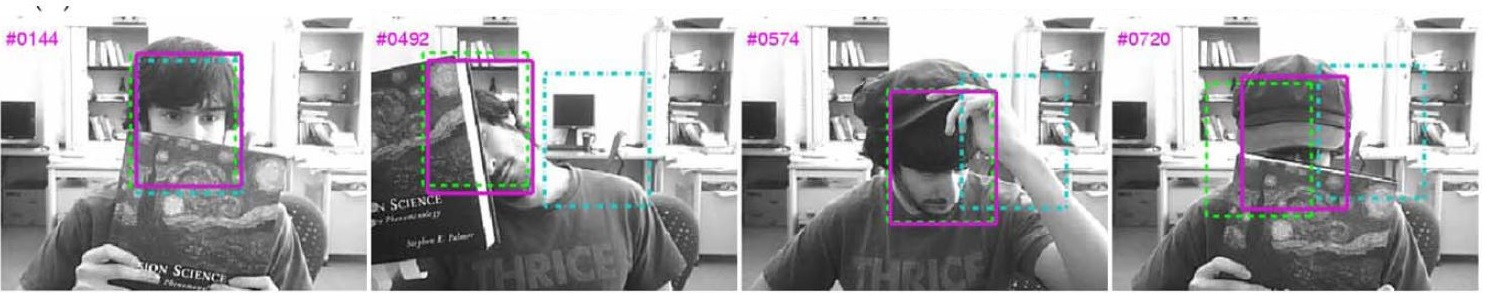
\includegraphics[width=1\linewidth]{images/tracking/sample_MIL}
	\captionsetup{margin=0.5cm}
	\caption[Examples of partial occlusion tracking.]{A sample of the MIL classifier tracking the face of the author while is partially occluded by a book. MIL tracker is in purple, while cyan and green are respectively FragTrack\cite{fragTrack} and Online Ada-Boost\cite{onlineAdaBoostTracker}.}
	\label{fig:sample_MIL}
\end{figure}
\begin{figure}[!h]
	\centering
	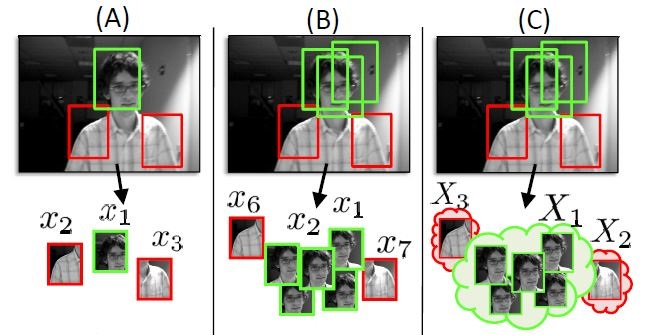
\includegraphics[width=0.8\linewidth]{images/tracking/howItWorks_MIL}
	\captionsetup{margin=0.5cm}
	\caption[The bag of bounding boxes introduced as MIL novelty.]{A comparison of how positive and negative samples are selected, to train the online classifier. In A the selection of BOOSTING tracker, the positive sample is used. In B a set of proposals generated around the positive are all used to train. In C the selection of MIL tracker, bags of samples are used and only one proposal is extracted and accepted from each one.}
	\label{fig:howItWorks_MIL}
\end{figure}


\subsection{KCF (Kernelized Correlation Filters) tracker} \label{sec:kcf}
The KCF tracker\cite{kcf}\cite{kcf-withColor} is an additional extension of MIL tracker.\\
The key idea is that the sampled images are similar due to the subject that is repeated or thanks to the background that does not change extremely fast compared to the FPS of the video. This repetition of similar patterns can be used to optimize the operations and speed up the computation. The technical improvement comes from the application of the \textbf{FFT (Fast Fourier Transformations)}, which allows to apply the elaboration of images in an efficient manner.\\
The novelty introduced with KCF allows this algorithm to outperform both BOOSTING and MIL, in terms of accuracy and speed. The weakness of this chain of three methods is the full occlusion. None of them is able to deal with total occlusion that always causes the tracking failure.


\subsection{Median Flow tracker} \label{sec:medianflow}
The Median Flow tracker\cite{medianFlow} is a reliable method that locates the subject according to its trajectory. The key idea is that the algorithm recognises points in two subsequent frames. These points should be the same physical element in the real space.\\
The overall procedure is shown in~\Cref{fig:howItWorks_medianFlow}. The first step (\Cref{fig:howItWorks_medianFlow_points}) consists of the creation of a grid of points on the initial bounding box, and then the localization of these points in all the future frames. This connection through the frames helps to know the exact motion model of the tracked algorithm. The \textbf{Motion Model} ($MM$) is the combination of actual position ($x, y$) and velocity. It is defined with the angle or direction of motion ($\theta$) and the module of the speed ($s$). Essentially knowing how the subject is moving helps to predict where it will be in the near future.
$$MM = ((x, y), (\theta, s))$$
The interaction of the frames works as follows. Every time that a new frame is added, the knowledge of the motion model suggests where the subject can be located. Then, the key points are searched in this new image. Once they are found it is fundamental to check the consistency of the trajectories (\Cref{fig:howItWorks_medianFlow_trajectory}). Each new point is associated with the most similar already known physical point and vice versa. If this double matching is correct and the two points refer to the same physical element the trajectory is confirmed (point 1 in the figure), otherwise there is a misalignment in the trajectories (point 2 in the figure). In~\Cref{fig:howItWorks_medianFlow_trajectory} point 2 is firstly (forward pass) associated with the front wheel, in the frame after is linked to the back wheel since the other one is hidden from the street signal. The backward pass links the back wheel again on itself. This misalignment of the connection is recognised as an error and so the point cannot be trusted. If no point can be trusted the tracking fails.\\
\\
Thanks to this double-checking procedure, the Median Flow tracker is a method that is able to well recognise when the tracking has failed to follow the subject. Unfortunately, the requirement to match key points over and over in the frames reduces the capability of the algorithm to manage scenarios where the subject appearance change too much.\\
For this reason, this algorithm is not good for tracking high deformable subjects such as animals and humans.

\begin{figure}[!h]
	\centering
	\begin{subfigure}{0.49\textwidth}
		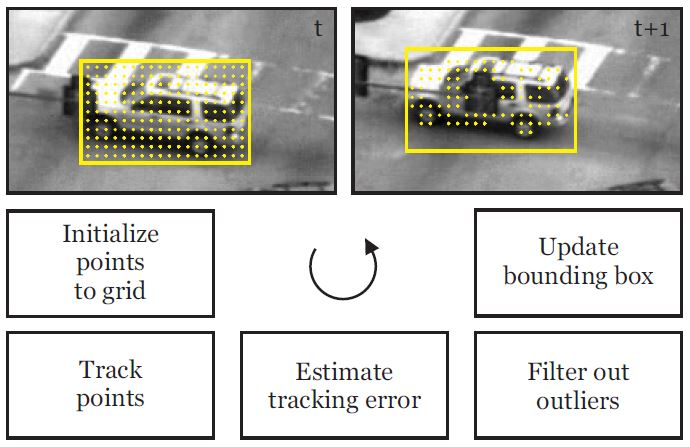
\includegraphics[width=\linewidth]{images/tracking/howItWorks_medianFlow_points}
		\captionsetup{margin=0.5cm}
		\caption{The first bounding box is divided into a grid of points, and a portion of them are recognised in the next frame. Below, the main steps of the algorithm.}
		\label{fig:howItWorks_medianFlow_points}
	\end{subfigure}
	\begin{subfigure}{0.49\textwidth}
		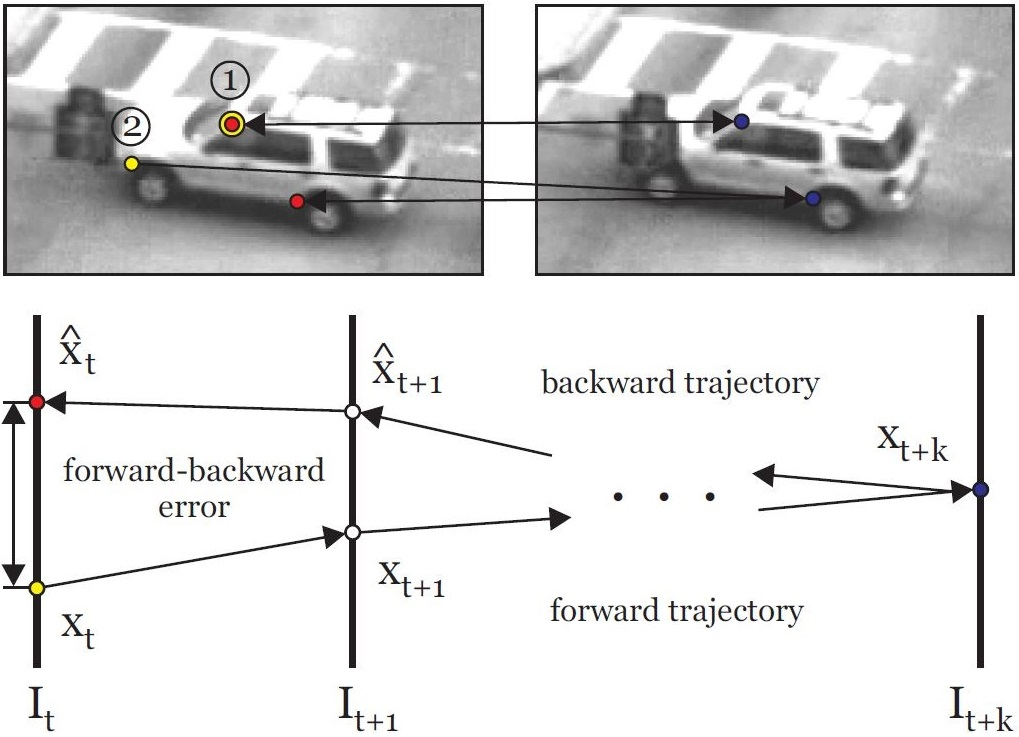
\includegraphics[width=\linewidth]{images/tracking/howItWorks_medianFlow_trajectory}
		\captionsetup{margin=0.5cm}
		\caption{The points found in two consecutive steps are compared to check if the forward and backward trajectories are the same and then it can be trusted.\\ Point 1 is accepted while point 2 is rejected.}
		\label{fig:howItWorks_medianFlow_trajectory}
	\end{subfigure}
	\captionsetup{margin=0.5cm}
	\caption[The key principle of the Median Flow tracker algorithm.]{The overall procedure of the Median Flow tracker computing forward and backward trajectories to precisely locate the target.}
	\label{fig:howItWorks_medianFlow}
\end{figure}


\subsection{CSRT (Channel and Spatial Reliability Tracker)}
The full name of the method is Discriminative Correlation Filter with Channel and Spatial Reliability (DCF-CSR)\cite{csrt}. Such as KCF (\Cref{sec:kcf}) and others, even this method is based on correlation filters.\\
\\
A \textbf{cross correlation filter} is a technique that aims at localizing into an image the exact position of another one. A representation of the cross-correlation usage done by CSRT is shown in~\Cref{fig:howItWorks_CSRT}. In details, the portion of the last frame, delimited by the last known bounding box, is elaborated with multiples correlation filters, each one producing a different output. These elaborations simulate possible changes in the appearance of the subject. Designing good filters is fundamental to well match the variability of the tracked subject and the generated features. The filter outputs are modified images of the last bounding box cropped area.\\
The output of each filter (an image) is moved along the full picture pixel by pixel (learning stage:~\Cref{fig:howItWorks_CSRT} left) to check which portion of the entire camera view is more probable the subject that we are looking for. The result of this scan is a confidence map that should present a peak in correspondence of the new position of the tracked subject.\\
All the filters can then be summed up together (localization stage:~\Cref{fig:howItWorks_CSRT} right) to highlight the proposal of each one and comes out with the final response. This response shows exactly where the subject is placed in the new frame. A visualization of a confidence map applied to the original image is shown in~\Cref{fig:sample_CSRT}.\\
\\
The characterization of CSRT is focused on the type of correlation filters used, with the idea of using a lot of them and combine the results at the end to produce a more reliable localization. The very high accuracy that this algorithm offers is compensated by the low FPS rate that it achieves.

\begin{figure}[!h]
	\centering
	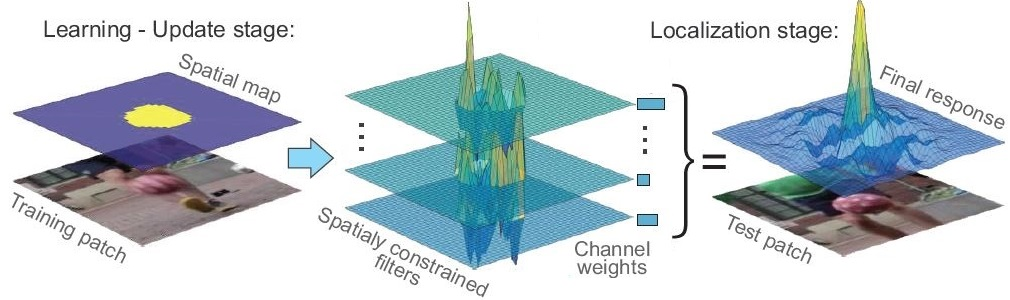
\includegraphics[width=1\linewidth]{images/tracking/howItWorks_CSRT}
	\captionsetup{margin=0.5cm}
	\caption[The general intuition of the CSRT algorithm.]{The overall procedure of the CSRT algorithm. The \underline{learning stage} is composed of multiple correlation filters that are applied to the input frame. Each filter produces a confidence map that highlights where the subject should be. The \underline{localization stage} combines all these confidence maps to produce the final response that precisely locates the subject.}
	\label{fig:howItWorks_CSRT}
\end{figure}
\begin{figure}[!h]
	\centering
	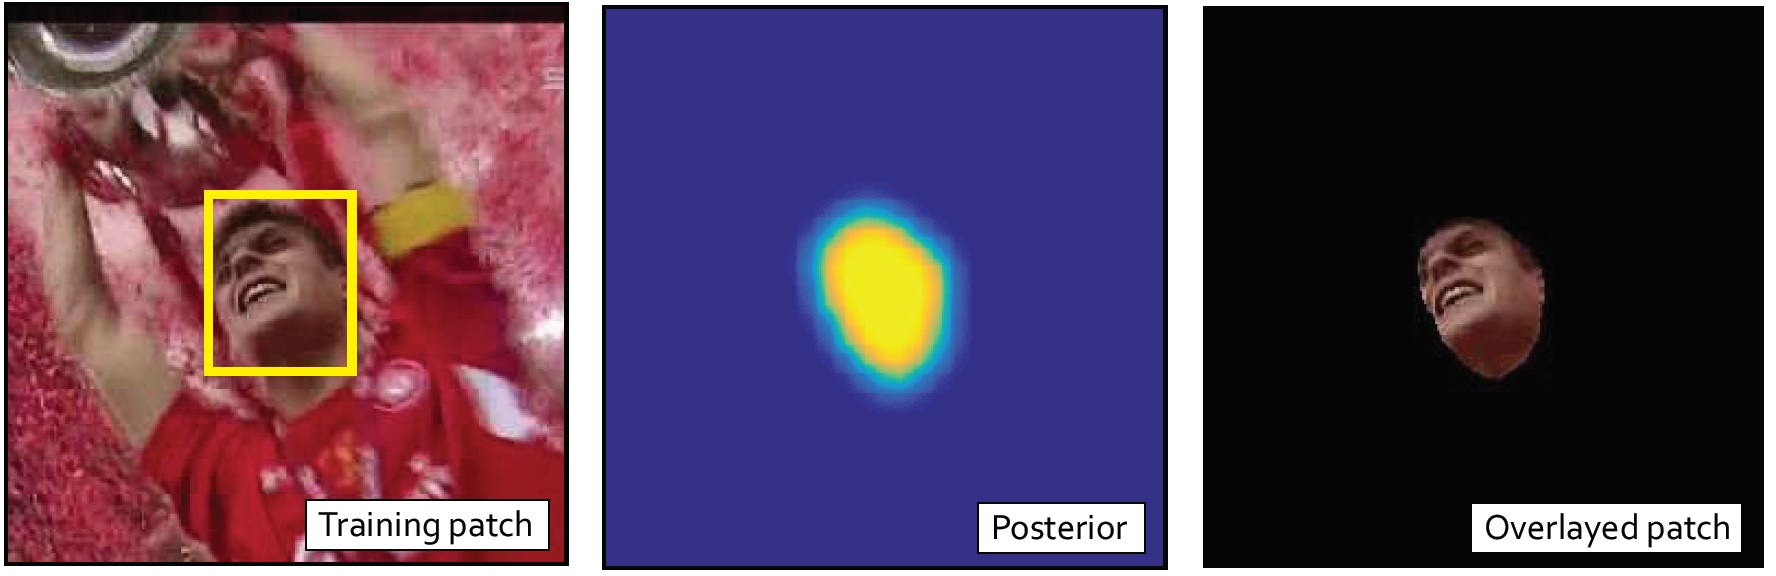
\includegraphics[width=0.8\linewidth]{images/tracking/sample_CSRT}
	\captionsetup{margin=0.5cm}
	\caption[An example of application of CSRT on a frame.]{A visualization of the confidence map applied to track the face of the man in the image. On the left the original image, centre the confidence map in 2D. On the right the cropped image according to localization.}
	\label{fig:sample_CSRT}
\end{figure}


\subsection{MOSSE (Minimum Output Sum of Squared Error) tracker}
The MOSSE algotihm\cite{mosse} such as KCF (\Cref{sec:kcf}) is a method whose strength lies into mathematical smart choices instead of a complex high-level logic like MedianFlow (\Cref{sec:medianflow}).\\
The novelty is introduced with a new correlation filter, called MOSSE. It can be applied to the input frames and precisely locate the variations fundamental to understand the movement of the subject.\\
Despite the original article states robustness against variations in lighting, scale and non-rigid deformations, this algorithm is not so reliable as it appears. On the other hand, the strength of this method is the extremely fast computations (FPS rate) that outperform all the other trackers presented in this section.

\subsection{GOTURN (Generic Object Tracking Using Regression Networks)} \label{sec:goturn}
GOTURN\cite{goturn} is a tracker based on neural networks. Differently from MIL and KCF (\Cref{sec:kcf}), this method is not based on an online NN, such as the online classifier, but it is based on an offline CNN.\\
An \textbf{offline NN} is a traditional NN that is trained on thousands of data: couples of images, in this case, producing the trained model. The process is done in advance, before the effective use, and not "on the fly" while running the tracker. The generated model is used at run time to know how to respond to an input value. The big advantage of offline methods is that the training procedure is the slowest section, for this reason an online classifier could not perform at very high FPS rates.\\
\\
The general workflow of the tracker is shown in~\Cref{fig:howItWorks_GOTURN}. The tracker takes as input a frame at a time and always compares it to the previous frame. This choice simplifies and standardizes the input to empower the potentiality of the CNN. However but makes the algorithm to have no chance against total occlusions even for one single frame. The CNN takes as input two squared images cropped from the frames. The crop on the previous frame is a bounding box centred around the last known position with some margins that will contain even the location in the frame afterwards. The current frame is cropped based on the same bounding box, but in this case, the subject is not centred in the square.\\
Then, both squared images are processed with two independent stacks of convolutional layers, followed by three fully-connected layers. The final output is composed of four values representing the top-left and bottom-right corners of the bounding box. It is centred on the subject in the squared image of the current frame. Some examples of the application of the CNN are shown in~\Cref{fig:sample_GOTURN}.

\begin{figure}[!h]
	\centering
	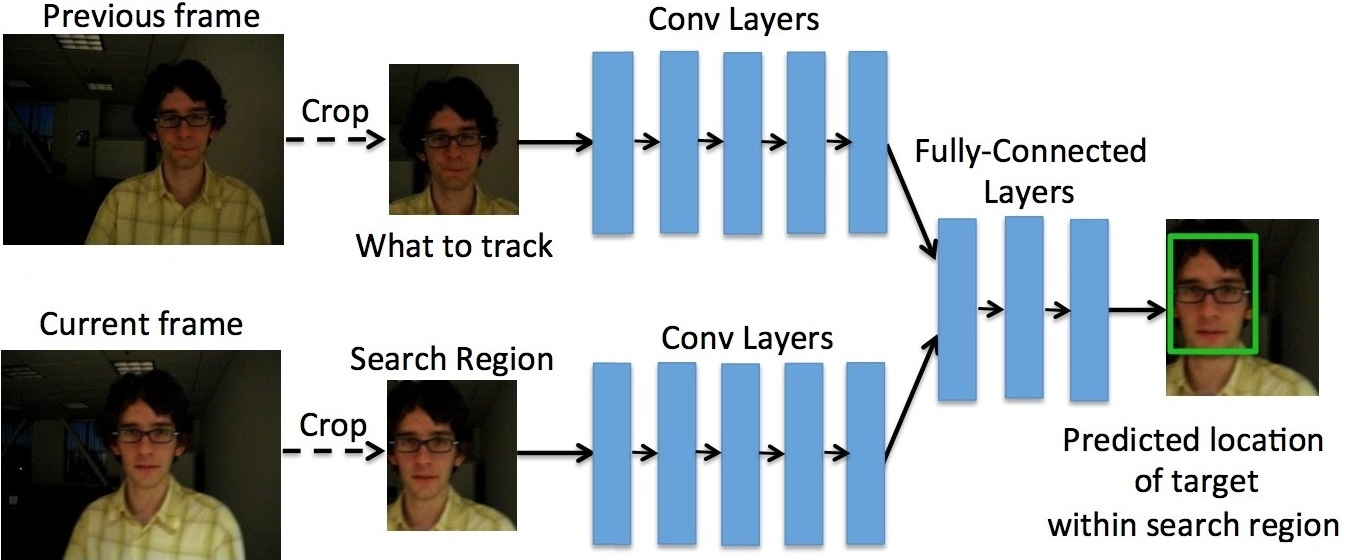
\includegraphics[width=1\linewidth]{images/tracking/howItWorks_GOTURN}
	\captionsetup{margin=0.5cm}
	\caption[The overall procedure of the GOTURN algorithm.]{The overall procedure of the GOTURN algorithm. On the left, the frames coming from the camera are cropped with the same square, that is centred on the subject in the previous frame (above). The images are elaborated with CNN to produce the output bounding box, that highlights where the subject is in the current frame.}
	\label{fig:howItWorks_GOTURN}
\end{figure}
\begin{figure}
	\centering
	\begin{minipage}{.65\textwidth}
		\centering
		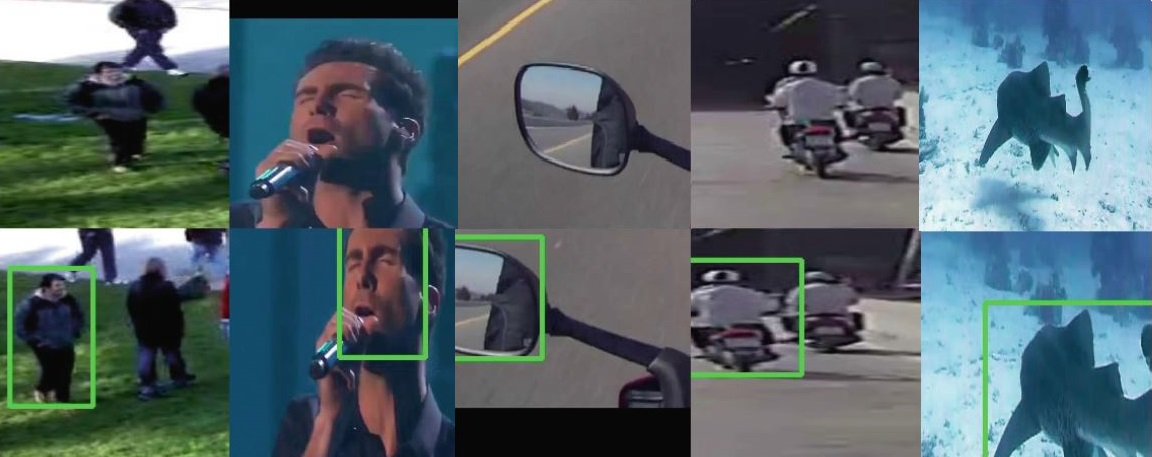
\includegraphics[width=1\linewidth]{images/tracking/sample_GOTURN}
		\captionsetup{margin=0.5cm}
		\captionof{figure}[Examples of application of the GOTURN algorithm.]{Samples of application of the CNN of GOTURN. The two squared images coming from previous (above) and current (below) frame are fed into the network. The answer is the green bounding box that locates the tracked subject on the new frame.}
		\label{fig:sample_GOTURN}
	\end{minipage}
	\begin{minipage}{.34\textwidth}
		\centering
		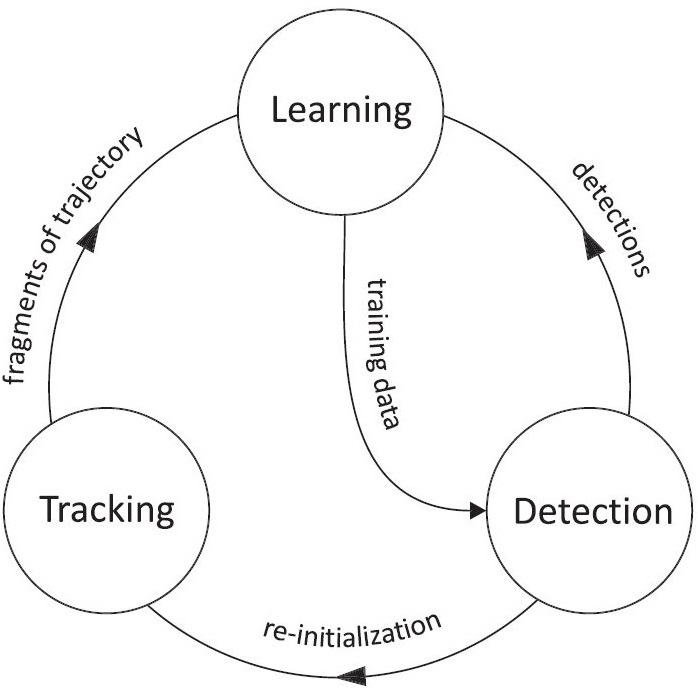
\includegraphics[width=1\linewidth]{images/tracking/howItWorks_TLD}
		\captionof{figure}{The interconnection of the three foundation methods of TLD algorithm.}
		\label{fig:howItWorks_TLD}
	\end{minipage}
\end{figure}

\subsection{TLD (Tracking-Learning-Detection)}
Differently from all the other methods, TLD\cite{tld} aims to be a complete tracker able to deal with extremely complex scenarios. If the previously presented trackers have no chance to manage a long-time total occlusion and a long-term tracking, this method is able to overcome both of the problems. A sample showing potentiality is in the~\Cref{fig:sample_TLD}.\\
The foundation principle is that TLD is not a single algorithm but it is a combination of three. The interaction of these three parts is shown in~\Cref{fig:howItWorks_TLD}. The key idea to overcome the re-identification problem that occurs after a total occlusion, or the drift problem that happens along a large video, is to often re-initialize the tracker. In fact, the \underline{tracking} (\textbf{T}) of TLD aims at managing short-term video clips. When a small problem occurs the \underline{detection} (\textbf{D}) tries to locate the subject back again. While these two situations take turns, the \underline{learning} procedure (\textbf{L}) extracts the key elements that recognise uniquely the subject and understand how to precisely locate it inside the frame.\\
\\
The trade-off to use this extremely flexible structure is paid with a not high FPS rate. However, the biggest problem of this method is the huge quantity of false-positive predictions. The learning procedure starts with a few samples, meaning that errors in the beginning phase can occur easily. The failure in the first phase causes wrong learning that will produce more and more errors later on.\\
Despite the good potentialities, this algorithm is not reliable for the traditional tracking task.
\begin{figure}[!h]
	\centering
	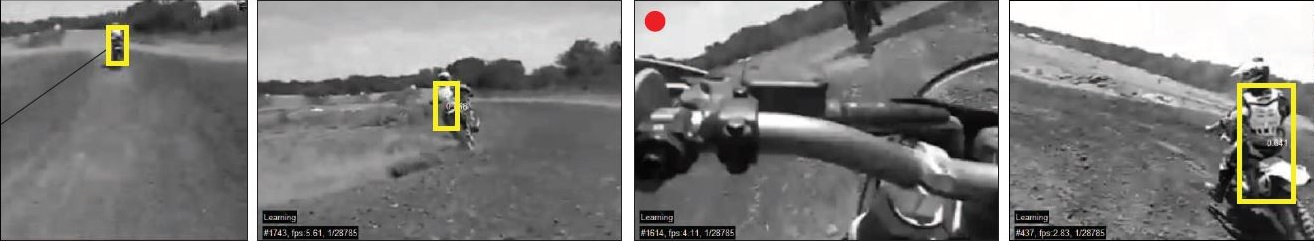
\includegraphics[width=1\linewidth]{images/tracking/sample_TLD}
	\captionsetup{margin=0.5cm}
	\caption[TLD algorithm applied on a total occlusion video clip.]{A sample that shows the potentialities of the TLD algorithm, dealing with a total occlusion while tracking a motorbike with a dramatic change of size. The red dot means that the subject cannot be found.}
	\label{fig:sample_TLD}
\end{figure}



\section{Which tracker could be chosen}
In the previous section we have presented seven different tracking algorithms, each one with his own strengths and weaknesses. These methods are the ones that were explored during this thesis work, but many others exist.\\
The tracking task that we aim at solving is a long real-time sequence with long-lasting total occlusions, as explained in~\Cref{sec:trackingBaseliveVsThesis}. This task is solved with a combination of detection, tracking and recognition, so the internal tracking challenge is much simpler.\\
The requirement is to solve the baseline tracking task (\Cref{sec:tracking-definition}), and to deal with changes of shape and partial occlusions. Considered the explained methods and known their speed performances (shown in~\Cref{tab:trackersFPS}), here it is what we have chosen. Note that the underlined methods are the best trade-off choices. 
\begin{itemize}
	\item \textbf{MIL tracker} is not a good choice because it runs at few FPS and a newer version that outperforms both its speed and accuracy exists.
	\item \underline{\textbf{KCF tracker}} is the new version of MIL. It is one of the fastest methods and it is also reliable. It suffers the rapid change of appearance and, less important for our scenario, it does not manage total occlusions.
	\item \textbf{Median Flow tracker} works well only on not deformable or rigid subjects. Since we are dealing with humans it is a bad choice.
	\item \underline{\textbf{CSRT}} is the most reliable method, it could even manage short total occlusions. Despite the low FPS rate is a great choice, in fact, our goal is a tracker running at around 5 FPS that is way less than the speed of CSRT.
	\item \underline{\textbf{MOSSE}} is focused on pure speed. It is not the most reliable method but it can be a good choice to try to reach the highest FPS rate for the general challenge.
	\item \underline{\textbf{GOTURN}} is a reliable method, running at a good FPS rate. At the moment it is not integrated in this project but it can be a great choice for future improvements.
	\item \textbf{TLD} is a too complex method. It is able to solve long total occlusions but easily fails on simpler scenarios, by proposing a lot of false positives. It is not reliable at all for our purpose.\\
	TLD is based on a principle that is similar to the one proposed in this thesis. The integration of tracking and detection linked together with a third procedure: learning in case of TLD and person recognition for this project. Both algorithms aim at solving the total occlusion problem and the drift problem with a reinitialization of the tracker performed with an object detector. The key difference is the existence in this thesis of the slow start phase presented in Section??? TODO.
\end{itemize}

\begin{table}[]
	\centering
	\begin{tabular}{|c|c|c|c|c|c|c|c|}
		\hline
		Algorithm & MIL & KCF & MedianFlow & CSRT & MOSSE & GOTURN & TLD \\ \hline
		FPS  & 9   & 38  & 40         & 15   & 56    & 20     & 10  \\ \hline
	\end{tabular}
	\captionsetup{margin=0.5cm}
	\caption[The FPS rates of the tracking algorithms.]{An overview of the FPS rate of the trackers described. The performances were measured on an Intel Core i5 CPU and on an Nvidia Jetson TX2 GPU. The speeds measured are almost the same.}
	\label{tab:trackersFPS}
\end{table} 	\clearpage
      \chapter{Recognition} \label{cha:recognition} \clearpage
      \chapter{Solution} \label{cha:solution}
This chapter is focused on the integration of the three modules of this thesis: detection, recognition and tracking. The explanation is based on the flow of the code, with special attention at the choices done and implementation details. The source code of the entire project is available on github\cite{projectSourceCode}.

\section{Wrapper function: follow} \label{sec:follow}
The code is entirely managed with a single class called \textbf{Follower}. This structure only requires to be initialized and then calling a "\textit{follow}" method (\Cref{alg:follow}) every time a new frame needs to be processed.\\
The class internally loads a new frame \li{2} from the webcam or, optionally, from a stored video. Both the sources can be used in "real-time". In fact, if the video is used some frames are internally discarded to simulate the losing of images due to a slow processing rate. Therefore the class \textit{Follower} can be analysed with both real-time tests but also recorded experiments. This feature is useful to replicate scenarios where the code have failed.\\
\\
The wrapper method \textit{follow} has only one task. It measures the elapsed time from the beginning of the tracking \li{4} and, according to this parameter, the \textit{slow start} phase (\Cref{sec:slowStartPhase}) is executed \li{5}  if less than X seconds are gone. Otherwise, the \textit{track leader} phase (\Cref{sec:trackleaderPhase}) is called \li{7}.

\begin{lstlisting}[captionpos=b, 
	caption={It is the pseudocode of the wrapper function that should grab the new incoming frames and redirect them to the first or second phase according to the time elapsed from the tracking begin.}, 
	label=alg:follow
	]
follow() -> position:
	frame = grab_newFrame()
	
	if elapsedTime() > phase1_length: #phase 1
	%*$\lfloor$*)	position = slowStartPhase(frame)
	else:							  #phase 2
	%*$\lfloor$*)	position = followPhase(frame)

	return position
\end{lstlisting}


\section{First phase: slow start} \label{sec:slowStartPhase}
This function is a novelty that we have chosen to introduce to empower the performances of the overall algorithm. The pseudo code of this method is provided at~\Cref{alg:slowStartPhase} while an example is shown in~\Cref{fig:slowStart}.\\
This project, differently from the traditional trackers and similarly to TLD (\Cref{sec:tld}), is based on an online learning classifier. Hence this phase is designed to immediately train KNN a little bit. This first generated knowledge will be then increased in the \textit{track leader} phase. KNN can classify the representative points that come from the bounding boxes of people in new frames, only according to other representative points previously archived. The \textit{slow start} phase is used to collect all the bounding boxes used to create the set of positive representative points into the N-dimensional space of KNN.\\
This elaboration works based on the assumption that during this first phase "\ul{The leader is the most important visible person}". The \textit{slow start} computes the detection of the visible people \li{3} and if one or more exists\li{5}, the leader is chosen as the bounding box, with the biggest area\li{6}. The X and Y pixel coordinates are computed to be retrieved \li{7} and the leader's box is given to KNN \li{8}. Simultaneously, a negative sample is randomly picked up from a database and it is also given to KNN \li{9}. This double fed is done to train KNN with a balanced number of positive and negative samples, in order to exploit the potentialities shown in~\Cref{fig:knn_googleNet_s9n18}. The negative samples come from a custom version of the Market1501 dataset\cite{market1501}, called \textbf{NegativePeople}, that we have created ad hoc for this purpose.\\
\\
The \textit{slow start} phase is executed for a period that can last for 3 up to 20 seconds or more. The value of this hyper-parameter influence the size of samples known by KNN when the official track starts. The longer this phase the better. The default value is set to 5 seconds. Alternatively, another possibility is that the first phase can be interrupted after that X points are given to KNN, but this does not guarantee a precise slot of time so this variant was discarded.

\begin{lstlisting}[captionpos=b, 
	caption={It is the pseudocode of the first phase. The function \textit{slow start} computes only detections in order to train the KNN people classifier.}, 
	label=alg:slowStartPhase
	]
slowStartPhase(frame) -> position:
	position = default
	boxes = detector.detectPeople(frame)
	
	if len(boxes)>=1:
	%*$\mid$*)	box = biggestAreaBB(boxes)
	%*$\mid$*)	position = getPosition(box)
	%*$\mid$*)	knn.addPositive(box)
	%*$\lfloor$*)	knn.addNegative(pickOneNegative())
	
	return position
\end{lstlisting}
\begin{figure}
	\centering
	\begin{minipage}{.49\textwidth}
		\centering
		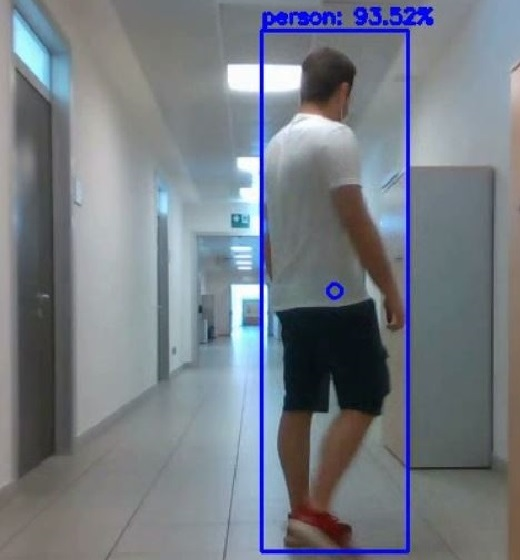
\includegraphics[width=1\linewidth]{images/solution/slowStart}
		\captionsetup{margin=0.2cm}
		\captionof{figure}[Frame of the slow start phase.]{Frame of the \textit{slow start} phase where the detection only is working. The leader has a \textbf{\textcolor{blue}{blue}} rectangle, and eventually other people are in \textbf{\textcolor{gray}{gray}}.}
		\label{fig:slowStart}
	\end{minipage}
	\begin{minipage}{.49\textwidth}
		\centering
		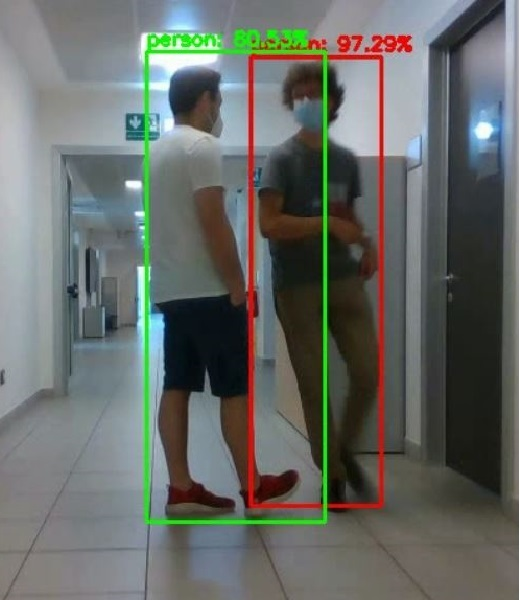
\includegraphics[width=1\linewidth]{images/solution/leaderSubjectOk}
		\captionsetup{margin=0.2cm}
		\captionof{figure}[A perfect detection example.]{A perfect detection where the two people are correctly recognised as leader (positive=\textbf{\textcolor{green}{green}}) and random person (negative=\textbf{\textcolor{red}{red}}).}
		\label{fig:doubleDetectionOk}
	\end{minipage}
\end{figure}


\section{Second phase: track leader} \label{sec:trackleaderPhase}
This function is the core of the entire project. The overall scheme of the pseudocode is shown at~\Cref{alg:trackleaderPhase}. In addition, in~\Cref{fig:sequenceTracking} there is a sequence of frames taken from a video clip where the robot is following the leader while it is shortly occluded twice by another person.\\
This phase works as follows:\\
\begin{itemize}
	\item The detection is performed \li{7} only one time every X frames \li{5}(details in~\Cref{sec:ratioDetectTrack}) and if the position of the leader is unknown \li{6}.\\
	The position is unknown immediately after the \textit{slow start} phase \li{2}, after the end of the tracking \li{29} and after a failed detection \li{17}.\\
	A sample detection over two people is shown in~\Cref{fig:doubleDetectionOk}.
	
	\item All the detections are elaborated \li{10} to check if are close to the last known position \li{11} and so can be kept or not (the drift optimization details are in~\Cref{sec:driftOptimization}). In addition, the KNN classifier is used \li{12} to accurately understood which detections contain the leader and which not (errors tolerance explained in~\Cref{sec:knnToleranceToFN}).\\
	Then, the false predictions are added to KNN \li{15}, while the positive ones are stored for more controls \li{13}.
	
	\item All the boxes that seem to contain the leader are further analysed \li{17-18}. The official prediction is chosen as the closest feasible box to the last known position \li{19} (more details in~\Cref{sec:multipleleaders}). Based on this final choice the tracked is re-initialized \li{20}.
	
	\item The new position is computed \li{22} and the elaborated bounding boxes are stored into KNN according to their content \li{23-24}. If only one detection was initially found \li{25}, and it was the leader, KNN is fed with a negative sample \li{26} coming from the NegativePeople dataset.
	
	\item After the initialization, the tracking is updated with new frames, one at a time \li{30}. The retrieved bounding box once converted into a position \li{31} is returned to the \textit{follow} function, both for detection and tracking \li{33}.
\end{itemize}
Special conditions and key aspects to focus on, follow in the next sections.

\begin{lstlisting}[captionpos=b, 
	caption={It is the pseudocode of the second phase. The function \textit{track leader} alternatively runs the detection and tracking modules to constantly know the position of the leader.}, 
	label=alg:trackleaderPhase
	]
trackleaderPhase(frame) -> position:
	static stopDetections = False
	position = default
	
	if onceEveryKTimes(10) 
	%*$\mid$*)  and not stopDetections: 					 #detection
	%*$\mid$*)	boxes = detector.detectPeople(frame)
	%*$\mid$*)	
	%*$\mid$*)	boxesOfleader = []
	%*$\mid$*)	foreach box in boxes:
	%*$\mid$*)	%*$\mid$*)	if checkDriftProximity(box)	  #drift optimization
	%*$\mid$*)	%*$\mid$*)	%*$\mid$*)   and knn.classify(box)==positive: #recognition
	%*$\mid$*)	%*$\mid$*)	%*$\lfloor$*)	 boxesOfleader.add(box)
	%*$\mid$*)	%*$\mid$*)	else:
	%*$\mid$*)	%*$\lfloor$*)	%*$\lfloor$*)	knn.addNegative(box)
	%*$\mid$*)			
	%*$\mid$*)	stopDetections = (len(boxesOfleader) > 0)
	%*$\mid$*)	if stopDetections:
	%*$\mid$*)	%*$\mid$*)	boxOfleader = pickClosestPosition(boxesOfleader) 
	%*$\mid$*)	%*$\mid$*)	tracker.initialize(frame, boxOfleader)
	%*$\mid$*)	%*$\mid$*)	
	%*$\mid$*)	%*$\mid$*)	position = getPosition(boxOfleader)
	%*$\mid$*)	%*$\mid$*)	knn.addPositive(boxOfleader)			 
	%*$\mid$*)	%*$\mid$*)	knn.addNegative(boxesOfleader except boxOfleader)
	%*$\mid$*)	%*$\mid$*)	if len(boxes) == 1:
	%*$\mid$*)	%*$\lfloor$*)	%*$\lfloor$*)	knn.addNegative(pickOneNegative())
	%*$\lfloor$*)		
	else: 										 #tracking
	%*$\mid$*)	stopDetections = False
	%*$\mid$*)	box = tracker.updateRegion(frame)
	%*$\lfloor$*)	position = getPosition(box)
	
	return position
\end{lstlisting}
\begin{figure}[!h]
	\centering
	\begin{subfigure}[!h]{0.325\textwidth}
		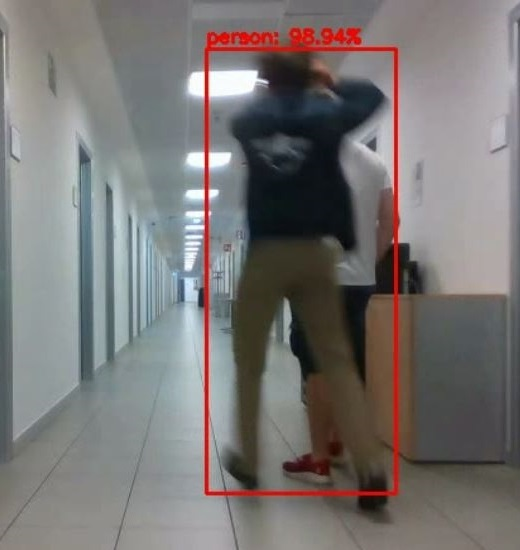
\includegraphics[width=\linewidth]{images/solution/sequenceTrackOk1}
	\end{subfigure}
	\begin{subfigure}[!h]{0.325\textwidth}
		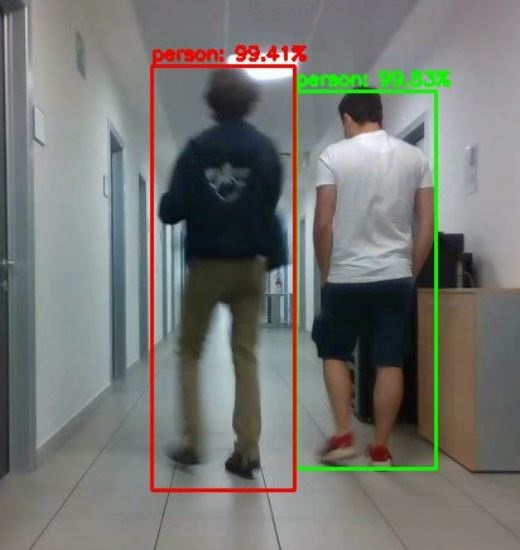
\includegraphics[width=\linewidth]{images/solution/sequenceTrackOk2}
	\end{subfigure}
	\begin{subfigure}[!h]{0.325\textwidth}
		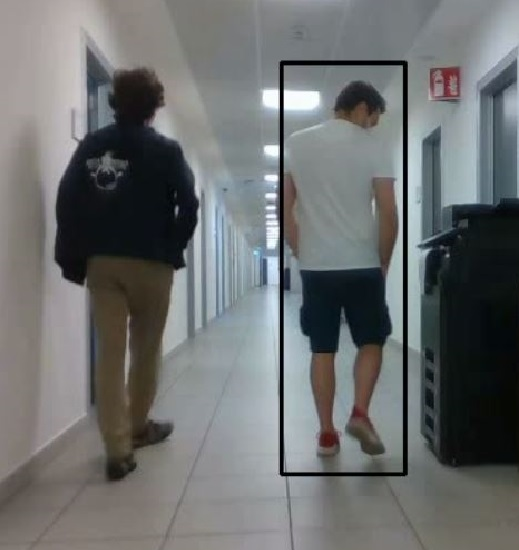
\includegraphics[width=\linewidth]{images/solution/sequenceTrackOk3}
	\end{subfigure}
	%
	\begin{subfigure}[!h]{0.325\textwidth}
		\includegraphics[width=\linewidth]{images/solution/sequenceTrackOk6}
	\end{subfigure}
	\begin{subfigure}[!h]{0.325\textwidth}
		\includegraphics[width=\linewidth]{images/solution/sequenceTrackOk7}
	\end{subfigure}
	\begin{subfigure}[!h]{0.325\textwidth}
		\includegraphics[width=\linewidth]{images/solution/sequenceTrackOk8}
	\end{subfigure}
	%
	\begin{subfigure}[!h]{0.325\textwidth}
		\includegraphics[width=\linewidth]{images/solution/sequenceTrackOk9}
	\end{subfigure}
	\begin{subfigure}[!h]{0.325\textwidth}
		\includegraphics[width=\linewidth]{images/solution/sequenceTrackOk10}
	\end{subfigure}
	\begin{subfigure}[!h]{0.325\textwidth}
		\includegraphics[width=\linewidth]{images/solution/sequenceTrackOk11}
	\end{subfigure}
	\captionsetup{margin=0.5cm}
	\caption[A video clip frames sequence of the tracking.]{A sequence of images representing a video clip while the robot is following the leader. The coloured rectangles in the images have different meanings. \textbf{\textcolor{green}{Green}} is the detection recognised as the leader. \textbf{\textcolor{red}{Red}} is a detection recognised as a not important person. \textbf{Black} is the tracker while following the leader.\\
		In this sample the leader is hidden twice and both times the algorithm is able to detect it back again and continue the tracking.}
	\label{fig:sequenceTracking}
\end{figure}


\subsection{Detection and tracking ratio} \label{sec:ratioDetectTrack}
It is fundamental to precisely define the alternation of the detection and the tracking along with the execution of the general method. This calibration is a trade-off among processing speed and localization accuracy. As shown in~\Cref{tab:detectionPerformances} and in~\Cref{tab:trackersFPS} the processing speed of the two modules is completely different. The detection is much slower compared to the tracking. Therefore, the highest FPS rate is reached with a tracker only solution, on the other hand, the highest localization accuracy is achieved with detection only technique. Note that with only detection and multiple subjects, the leader is identified thanks to the recognition module.\\
The disclaimer is to choose the minimum required FPS rate and then hope that the accuracy is enough. In our case, we have fixed $5$ FPS as a target. To respect this limit the detection is executed once every $10$ processed frames. It is important to remember that if a single detection fails or the leader is not found, the tracker cannot be started. Consequently, from that moment on all the frames are processed with the detection. This recovery procedure will run at low FPS but the leader is momentarily lost, so, it is not important.\\
\\
If the high FPS needs to be reached the solution may consist of changing this mechanic. The detector might be started only after the tracker reports that it lost the leader. This will reduce the number of detections and improve the overall FPS rate. Unfortunately, a lot of trackers are not precisely able to recognize when the tracked subject has been lost, hence the implementation is not straightforward, and at the moment has not been written yet.


\subsection{Drift tolerance optimization} \label{sec:driftOptimization}
The idea of this optimization comes from two conditions that should be managed. On one hand, the drift problem that is one of the main weaknesses of the trackers, in fact over a long video sequence it can be a huge problem. On the other hand, the proximity assumption (\Cref{fig:challenge_proximity}) that allows the tracked subject to move only for a limited number of pixels per frame.\\
These two conditions combined can be used to wisely classify the new detections once the tracker has been stopped. If a new detection is too far away compared to the last known position of the leader, it cannot be the leader itself. Otherwise, the recognition module should be used to normally predict the class of the new bounding box.\\
We have defined the tolerance of the movement as:
$$d = t\cdot s\cdot\left(\frac{w}{100}\right)^{2}$$
In the above formula the symbols represent:
\begin{itemize}
	\item \textbf{d} is the distance allowed.
	\item \textbf{t} is the time elapsed from the last correct detection of the leader. It is used to manage the drift problem independently of the ratio between tracking and detection.
	\item \textbf{s} is an empirical scale factor, experimentally measured to be around $0.05$. It is the hyper-parameter to manage this optimization. 
	\item \textbf{w} is the width of the last bounding box during the tracking. It is used to simulate the distance of the leader from the camera. Compared to a far detection, a close leader has a bigger bounding box hence the multiplying factor is greater. This difference is fundamental to manage the fast 2D movement of a close subject.
\end{itemize}
In~\Cref{fig:driftOptimizationFail} is shown an example where a person is immediately classified as negative because it is too far away. Instead, in~\Cref{fig:driftOptimizationOk} the person is inside the tolerance and further analysis with KNN has classified this person as the leader.

\begin{figure}[!h]
	\centering
	\begin{subfigure}[!h]{0.49\textwidth}
		\includegraphics[width=\linewidth]{images/solution/driftOptimizationFail}
		\captionsetup{margin=0.5cm}
		\caption{The person is classified as Negative because it is outside of the \textit{drift tolerance} circle.}
		\label{fig:driftOptimizationFail}
	\end{subfigure}
	\begin{subfigure}[!h]{0.39\textwidth}
		\includegraphics[width=\linewidth]{images/solution/driftOptimizationOk}
		\caption{The person is classified as Positive because it is outside of the \textit{drift tolerance} circle.}
		\label{fig:driftOptimizationOk}
	\end{subfigure}
	\captionsetup{margin=1.4cm}
	\caption[Two samples of the \textit{drift tolerance} optimization.]{Two samples of the \textit{drift tolerance} optimization represented as a \textbf{\textcolor{orange}{yellow}} circle, centred on the last known position (a small black circle).}
	\label{fig:driftOptimization}
\end{figure}

\subsection{Multiple leaders corner case} \label{sec:multipleleaders}
It may happen that there are two people both inside the \textit{drift tolerance} circle and both are classified as the leader from KNN. This of course is real scenario impossible (a person cannot be duplicated) hence only one can be chosen as the right one. Further analysis can be used but we have chosen a simpler idea: \textit{"The closest subject to the last know position will be the official leader"}.\\
In~\Cref{fig:leaderSubjectDoubleMatch} there is a sample scenario registered before the introduction of this elaboration.
\begin{figure}
	\centering
	\begin{minipage}{.49\textwidth}
		\centering
		\includegraphics[width=1\linewidth]{images/solution/leaderSubjectDoubleMatch}
		\captionsetup{margin=0.2cm}
		\captionof{figure}[A frame with two leaders.]{A failed scenario where the two people are recognised both as leader, instead one is a random person.}
		\label{fig:leaderSubjectDoubleMatch}
	\end{minipage}
	\begin{minipage}{.49\textwidth}
		\centering
		\includegraphics[width=1\linewidth]{images/solution/leaderSubjectDoubleFail}
		\captionsetup{margin=0.2cm}
		\captionof{figure}[A frame with two random people.]{A failed scenario where the two people are recognised both as random people, instead one is the leader.}
		\label{fig:leaderSubjectDoubleFail}
	\end{minipage}
\end{figure}

\subsection{KNN tolerance against false-negative} \label{sec:knnToleranceToFN}
The previous section introduces the failure of the KNN classifier that predicts a leader in exceed. This is a false-positive classification. As explained this is miss prediction can be managed. On the other hand, a false-negative classification is a much bigger problem. It happens when the leader is classified as negative, an example is shown in~\Cref{fig:leaderSubjectDoubleFail}.\\
This wrong prediction is complex because, after the classification, the generated representative point and its new label are fed into KNN. This false-negative represent a point wrongly classified. However, also a false-positive is fed into KNN but if there are multiple leaders further analysis can reduce them. Instead, a leader classified as negative cannot be re-evaluated hence it cannot be converted into a correct prediction, it will be an error forever.\\
Due to the mechanics of KNN, a small set of wrong classified points can cause a lot of wrong classifications in future analysis. Therefore we absolutely want to avoid false-negative predictions. 	\clearpage
      \chapter{Conclusion} \label{cha:conclusion} 	\clearpage
      
      
    \endgroup


    % bibliografia in formato bibtex
    %
    % aggiunta del capitolo nell'indice
    \addcontentsline{toc}{chapter}{Bibliografia}
    % stile con ordinamento alfabetico in funzione degli autori
    \bibliographystyle{unsrt}
    \bibliography{biblio}
%%%%%%%%%%%%%%%%%%%%%%%%%%%%%%%%%%%%%%%%%%%%%%%%%%%%%%%%%%%%%%%%%%%%%%
%%%%%%%%%%%%%%%%%%%%%%%%%%%%%%%%%%%%%%%%%%%%%%%%%%%%%%%%%%%%%%%%%%%%%%
%% Nota
%%%%%%%%%%%%%%%%%%%%%%%%%%%%%%%%%%%%%%%%%%%%%%%%%%%%%%%%%%%%%%%%%%%%%%
%% Nella bibliografia devono essere riportati tutte le fonti consultate 
%% per lo svolgimento della tesi. La bibliografia deve essere redatta 
%% in ordine alfabetico sul cognome del primo autore. 
%% 
%% La forma della citazione bibliografica va inserita secondo la fonte utilizzata:
%% 
%% LIBRI
%% Cognome e iniziale del nome autore/autori, la data di edizione, titolo, casa editrice, eventuale numero dell’edizione. 
%% 
%% ARTICOLI DI RIVISTA
%% Cognome e iniziale del nome autore/autori, titolo articolo, titolo rivista, volume, numero, numero di pagine.
%% 
%% ARTICOLI DI CONFERENZA
%% Cognome e iniziale del nome autore/autori (anno), titolo articolo, titolo conferenza, luogo della conferenza (città e paese), date della conferenza, numero di pagine. 
%% 
%% SITOGRAFIA
%% La sitografia contiene un elenco di indirizzi Web consultati e disposti in ordine alfabetico. 
%% E’ necessario:
%%   Copiare la URL (l’indirizzo web) specifica della pagina consultata
%%   Se disponibile, indicare il cognome e nome dell’autore, il titolo ed eventuale sottotitolo del testo
%%   Se disponibile, inserire la data di ultima consultazione della risorsa (gg/mm/aaaa).    
%%%%%%%%%%%%%%%%%%%%%%%%%%%%%%%%%%%%%%%%%%%%%%%%%%%%%%%%%%%%%%%%%%%%%%
%%%%%%%%%%%%%%%%%%%%%%%%%%%%%%%%%%%%%%%%%%%%%%%%%%%%%%%%%%%%%%%%%%%%%%
    

    %\titleformat{\chapter}
    %    {\normalfont\Huge\bfseries}{Allegato \thechapter}{1em}{}
    % sezione Allegati - opzionale
	%\appendix
    %\chapter{Titolo primo allegato}

Lorem ipsum dolor sit amet, consectetur adipiscing elit. Donec sed nunc orci. Aliquam nec nisl vitae sapien pulvinar dictum quis non urna. Suspendisse at dui a erat aliquam vestibulum. Quisque ultrices pellentesque pellentesque. Pellentesque egestas quam sed blandit tempus. Sed congue nec risus posuere euismod. Maecenas ut lacus id mauris sagittis egestas a eu dui. Class aptent taciti sociosqu ad litora torquent per conubia nostra, per inceptos himenaeos. Pellentesque at ultrices tellus. Ut eu purus eget sem iaculis ultricies sed non lorem. Curabitur gravida dui eget ex vestibulum venenatis. Phasellus gravida tellus velit, non eleifend justo lobortis eget. 

\section{Titolo}
Lorem ipsum dolor sit amet, consectetur adipiscing elit. Donec sed nunc orci. Aliquam nec nisl vitae sapien pulvinar dictum quis non urna. Suspendisse at dui a erat aliquam vestibulum. Quisque ultrices pellentesque pellentesque. Pellentesque egestas quam sed blandit tempus. Sed congue nec risus posuere euismod. Maecenas ut lacus id mauris sagittis egestas a eu dui. Class aptent taciti sociosqu ad litora torquent per conubia nostra, per inceptos himenaeos. Pellentesque at ultrices tellus. Ut eu purus eget sem iaculis ultricies sed non lorem. Curabitur gravida dui eget ex vestibulum venenatis. Phasellus gravida tellus velit, non eleifend justo lobortis eget. 

\subsection{Sottotitolo}
Lorem ipsum dolor sit amet, consectetur adipiscing elit. Donec sed nunc orci. Aliquam nec nisl vitae sapien pulvinar dictum quis non urna. Suspendisse at dui a erat aliquam vestibulum. Quisque ultrices pellentesque pellentesque. Pellentesque egestas quam sed blandit tempus. Sed congue nec risus posuere euismod. Maecenas ut lacus id mauris sagittis egestas a eu dui. Class aptent taciti sociosqu ad litora torquent per conubia nostra, per inceptos himenaeos. Pellentesque at ultrices tellus. Ut eu purus eget sem iaculis ultricies sed non lorem. Curabitur gravida dui eget ex vestibulum venenatis. Phasellus gravida tellus velit, non eleifend justo lobortis eget. 


\chapter{Titolo secondo allegato}

Lorem ipsum dolor sit amet, consectetur adipiscing elit. Donec sed nunc orci. Aliquam nec nisl vitae sapien pulvinar dictum quis non urna. Suspendisse at dui a erat aliquam vestibulum. Quisque ultrices pellentesque pellentesque. Pellentesque egestas quam sed blandit tempus. Sed congue nec risus posuere euismod. Maecenas ut lacus id mauris sagittis egestas a eu dui. Class aptent taciti sociosqu ad litora torquent per conubia nostra, per inceptos himenaeos. Pellentesque at ultrices tellus. Ut eu purus eget sem iaculis ultricies sed non lorem. Curabitur gravida dui eget ex vestibulum venenatis. Phasellus gravida tellus velit, non eleifend justo lobortis eget. 

\section{Titolo}
Lorem ipsum dolor sit amet, consectetur adipiscing elit. Donec sed nunc orci. Aliquam nec nisl vitae sapien pulvinar dictum quis non urna. Suspendisse at dui a erat aliquam vestibulum. Quisque ultrices pellentesque pellentesque. Pellentesque egestas quam sed blandit tempus. Sed congue nec risus posuere euismod. Maecenas ut lacus id mauris sagittis egestas a eu dui. Class aptent taciti sociosqu ad litora torquent per conubia nostra, per inceptos himenaeos. Pellentesque at ultrices tellus. Ut eu purus eget sem iaculis ultricies sed non lorem. Curabitur gravida dui eget ex vestibulum venenatis. Phasellus gravida tellus velit, non eleifend justo lobortis eget. 

\subsection{Sottotitolo}
Lorem ipsum dolor sit amet, consectetur adipiscing elit. Donec sed nunc orci. Aliquam nec nisl vitae sapien pulvinar dictum quis non urna. Suspendisse at dui a erat aliquam vestibulum. Quisque ultrices pellentesque pellentesque. Pellentesque egestas quam sed blandit tempus. Sed congue nec risus posuere euismod. Maecenas ut lacus id mauris sagittis egestas a eu dui. Class aptent taciti sociosqu ad litora torquent per conubia nostra, per inceptos himenaeos. Pellentesque at ultrices tellus. Ut eu purus eget sem iaculis ultricies sed non lorem. Curabitur gravida dui eget ex vestibulum venenatis. Phasellus gravida tellus velit, non eleifend justo lobortis eget. 




\end{document}
